\documentclass[12pt,a4paper]{report}

\usepackage[utf8]{inputenc}
\usepackage[T1]{fontenc}

\usepackage[toc]{glossaries}

\usepackage[backend=biber,autocite=plain,sorting=ynt,ibidtracker=constrict]{biblatex}
\usepackage{csquotes}
\usepackage{hyperref}
\usepackage{caption}
\usepackage{labels}
\usepackage{pgf-pie}
\usepackage{makecell}

\usepackage[includefoot,a4paper, total={6.5in, 9.5in}]{geometry}

\usepackage{graphicx, copyrightbox}
\usepackage{appendix}
\usepackage{float}
\usepackage{subcaption}
\usepackage{pgf-pie}
\usepackage{tikz}

\setlength{\parindent}{24pt} 


\addbibresource{bib.bib}

\usepackage[french]{babel}


\title{MR 52 : Contraception masculine}
\author{Esteban BECKER}
\date{2023}
\begin{document}
\maketitle
\tableofcontents
\chapter*{Introduction}

\begin{figure}[h]
    \centering
    
\includegraphics[width=0.6\textwidth]{images/intro/choisir-sa-contraception.png}
    \caption{Brochure de santé publique France sur la contraception.}
    \label{fig:brochureSPF}
\end{figure}
On peut voir sur cette brochure de santé publique France qu'il y a uniquement 2 hommes représentés face à 10 femmes. \cite{santepublicfranceChoisirSaContraception2019}
\chapter{Les méthodes de contraception}

Il y a actuellement plusieurs méthodes de contraception disponible et en cours de développement à différents stades. Mais avant cela, qu'elles sont les critères d'une bonne méthode de contraception ?
On peut en citer 4 principaux :
\begin{itemize}
    \item sécurité : La méthode ne doit pas être dangereuse pour la santé
    \item Réversibilité : On doit pouvoir retrouver la fertilité qu'on avait avant son utilisation. Ce critère est sujet à discutions, en effet, une méthode irréversible peut être intéressante, mais va concerner moins de personnes.
    \item Efficacité : Une méthode doit être efficace pour éviter les grossesses non désirées.
    \item Acceptabilité : Une méthode doit être facile d'utilisation et être financièrement accessible. \cite{mieussetPotentialMildTesticular1994}
\end{itemize}

\section{Les méthodes de la Haute Autorité de Santé (HAS)}
Sur leur site, la haute autorité de santé liste 3 options de contraception masculine : le préservatif, la vasectomie et le retrait. \cite{ContraceptionChezHomme2019}

\subsection{Le préservatif}

\begin{figure}[h]
    \centering
    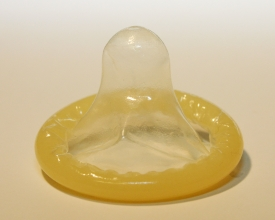
\includegraphics[width=0.3\textwidth]{images/scientiphique/Kondom.jpg}
    \caption{Préservatif masculin enroulé par User Flegmus sur pl.wikipedia — Flegmus, CC BY-SA 3.0, \href{https://commons.wikimedia.org/w/index.php?curid=1293908}{https://commons.wikimedia.org/w/index.php?curid=1293908}}
    \label{fig:preservatif}
\end{figure}

Le préservatif est une méthode de contraception consistant en un étui étanche. Il permet de séparer le sperme du vagin et ainsi d'éviter la fécondation. \cite{PreservatifWikipedia}
De plus, il est le moyen le plus efficace de se protéger des IST (infection sexuellement transmissible). \cite{MaladiesInfectionsSexuellement}
Le préservatif qui nous intéresse est le préservatif masculin moderne qui est principalement en latex et a été inventé en 1855. \cite{PreservatifWikipedia}
C'est le premier moyen de contraception recommander quand on a un nouveau partenaire sexuel ou un inconnu grâce à sa protection contre les IST. \cite{PreventionIST}
Son niveau d'efficacité théorique est de 98\% et son efficacité réelle est de 85\% selon l'indice de Pearl. L'indice de Pearl mesure l'efficacité d'une méthode de contraception, il s'agit du nombre de grossesses involontaires pour 100 femmes utilisant cette méthode pendant un an.\cite{EfficaciteMoyensContraceptifs}
Cette différence s'explique principalement par un mauvais emplois du préservatif.
Le préservatif doit être mis avant chaque rapport. \cite{TousMoyensContraception2023} 

\subsection{La vasectomie}

\begin{figure}[h]
    \centering
    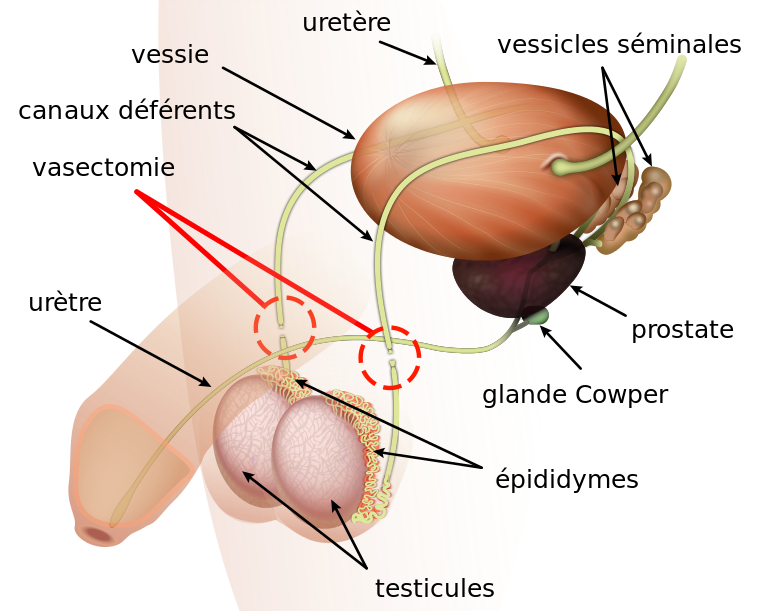
\includegraphics[width=0.5\textwidth]{images/scientiphique/Vasectomie_fr.svg.png}
    \caption{Schéma d'un pénis avec l'emplacement de la vasectomie par K. D. Schroeder, CC BY-SA 3.0, \href{https://commons.wikimedia.org/w/index.php?curid=41078528}{https://commons.wikimedia.org/w/index.php?curid=41078528}}
    \label{fig:vasectomie}
\end{figure}

Il ne faut pas confondre castration et vasectomie, la castration consiste à retirer les testicules alors que la vasectomie est une méthode de contraception consistant à sectionner les canaux déférents.
Il existe deux méthodes de vasectomie :
\begin{itemize}
    \item La technique classique (la méthode la plus courante) où le chirurgien effectue deux incisions au niveau du scrotum puis découpe une section des canaux déférents. Il termine l'opération par l'instalation de points de sutures ou d'agrafes \cites{VasectomieToutSavoir2017}{guillaumedaudinContraceptesEnqueteDernier2022}
    \item La technique sans bistouri où une pince spéciale permet d'extraire les canaux par un petit trou. Ce qui permet de ne pas faire d'incisions. Ensuite les canaux sont cousus cautérisé et découpé. Cette méthode de par les plus petites ouvertures ne nécessite pas de points de sutures et diminue les risques de complication. \cites{VasectomieToutSavoir2017}{guillaumedaudinContraceptesEnqueteDernier2022} Cela empêche les spermatozoïdes d'être présent dans le sperme mais n'a pas d'effet sur l'éjaculation.
\end{itemize}
L'opération se fait en une dizaine de minutes sous anesthésie locale. \cite{VasectomieEstelleReversible}
La vasectomie est autorisée en France depuis 2001. \cite{guillaumedaudinContraceptesEnqueteDernier2022} Pour effectuer une vasectomie, il faut avoir plus de 18 ans et après un délai de réflexion de 4 mois. C'est-à-dire qu'après un premier rendez-vous pour effectuer une vasectomie et où l'on a mis par écrit son souhait d'effectuer une vasectomie, il faut attendre 4 mois pour un second rendez-vous où l'on confirme son souhait d'effectuer une vasectomie. \cite{SterilisationViseeContraceptive}
Après la vasectomie, il faut respecter un délai de 12 semaines avant d'être stérile. \cite{associationfrancaisedurologieVasectomieContraceptive2012}. Son efficacité est de 99\% selon l'indice de Pearl. \cite{EfficaciteMoyensContraceptifs}
Cette méthode ne protège pas des IST.

La vasovasectomie est l'opération permettant de réparer une vasectomie. Il faut savoir qu'en France le taux de réussite dans les trois premières années est de 30 à 70 \% selon l'association française d'urologie et si l'on attend plus longtemps, le taux chute. Elle est donc à considérer comme une méthode définitive.\cite{VasectomieEstelleReversible}
Il faut savoir que la vasovasectomie est mieux réussi dans les pays où la vasectomie est plus régulièrement utilisé, en effet les médecins français ne sont pas habitué à effectuer des vasovasectomie. \cite{guillaumedaudinContraceptesEnqueteDernier2022}


\subsection{Le retrait} \label{section:leretrait}

Le retrait (ou coït interrompu) est une méthode de contraception consistant à retirer le pénis du vagin avant l'éjaculation. \cite{CoitInterrompuWikipedia}
Bien qu'efficace en théorie à 96\% elle ne l'est en pratique qu'à 78\%. \cite{TousMoyensContraception2023}
Contrairement à une idée reçu, le liquide pré-séminale ne contient pas de spermatozoïdes s'il n'y a pas eu une éjaculation récente. \cite{freeMaleContraceptionPrescription}
La faible efficacité vient de la difficulté à retirer le pénis au bon moment ou à une précédente éjaculation récente. \cite{CoitInterrompuWikipedia}
Elle est donc à considérer comme une méthode peu efficace et selon les professionnels de santé avec lesquels j'ai dialogué, elle ne doit pas être utilisé comme méthode de contraception.
Cette méthode ne protège pas des IST.

\section{Les méthodes non validés par la Haute Autorité de Santé}

Pour mieux comprendre comment est validés un médicament voir l'annexe \ref{annexe:etapes_recherche}.

\subsection{La contraception hormonale masculine}

Pour comprendre comment fonctionne la contraception hormonale masculine, il faut comprendre comment fonctionne la production de spermatozoïdes.
La production de spermatozoïdes est contrôlé par l'axe hypothalamo-hypophyso-gonadique. Il s'agit de la connexion entre l’hypothalamus, l’hypophyse et les gonades. \cite{HypothalamicPituitaryGonadal2022}
En fonction du taux de testostérone présent dans le corps l'hypothalamus va libérer des gonadotrophines (GnRH), ce qui va stimuler l'hypophyse. Qui elle a son tour va libérer l'hormone lutéinisante (LH) et l'hormone folliculostimulante (FSH).
La LH va stimuler les cellules de Sertoli pour lancer la spermatogenèse et produire des spermatozoïdes. La FSH va stimuler les cellules de Leydig pour produire de la testostérone. \cite{abbeMaleContraception2020}

\begin{figure}[h]
    \centering
    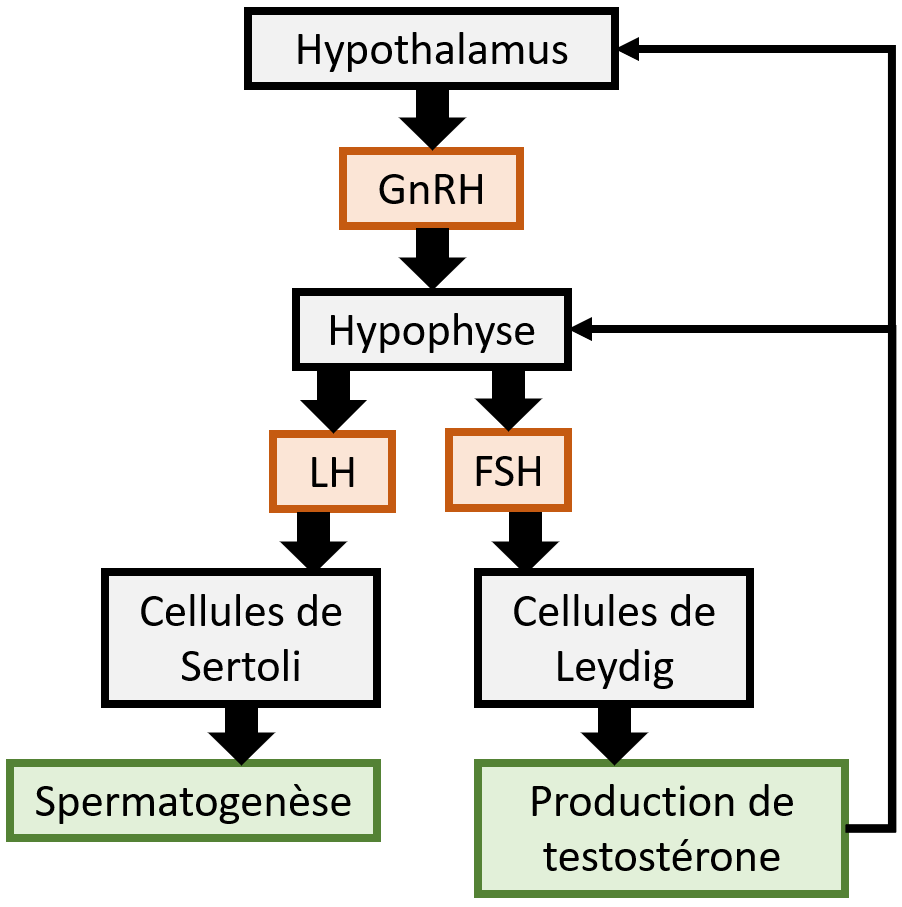
\includegraphics[width=0.4\textwidth]{images/scientiphique/axe-HPG.png}
    \caption{Schéma de l'axe hypothalamo-hypophyso-gonadique}
    \label{fig:axe-hypothalamo-hypophyso-gonadique}
\end{figure}

Ici les méthodes de contraception hormonale masculine vont viser à augmenter soit le taux de testostérone soit le taux de progestatif, ce qui va tromper l'hypothalamus et l'hypophyse et ainsi diminuer la production de spermatozoïdes. \cite{abbeMaleContraception2020}

\begin{figure}[h]
    \centering
    \includegraphics[width=0.7\textwidth]{images/scientiphique/axe-HPG-contracepté.png}
    \caption{Schéma de l'axe hypothalamo-hypophyso-gonadique avec une contraception hormonale masculine}
    \label{fig:axe-hypothalamo-hypophyso-gonadique-contracepte}
\end{figure}

La spermatogenèse étant un processus long, les méthodes hormonales ont un délai minimum de 3 mois entre la première prise et la stérilité. 

\subsubsection{La contraception hormonale par injection} \label{section:injection}

Il existe plusieurs méthodes de contraception hormonale masculine par injection :
\begin{itemize}
    \item L'injection intramusculaire de testostérone :
    \begin{itemize}
        \item 200 mg de testostérone hebdomadaire 
        \item 500 mg d’undécanoate de testostérone mensuelle (forme à libération prolongée) \cite{tcherdukianContraceptionMasculineQuelles2020}
    \end{itemize}
    \item L'injection intramusculaire de testostérone et de progestatif. Le progestatif permet de diminuer la production de spermatozoïdes et la testostérone est là pour compenser la diminution de la testostérone due au progestatif. \cite{longUpdateNovelHormonal2021}
\end{itemize}

Ainsi l'OMS a testé en 1990 l'injection intramusculaire de 200 mg d'enanthate de testostérone par semaines et dans une seconde étude de 196 avec 349 hommes. Les résultats sont positifs. En effet, sur la seconde étude l'indice de Pearson est de 1.4 grossesse. \cite{guerinContraceptionMasculineHormonale1996}
L'OMS a donc validé cette méthode de contraception, mais elle n'a pas autorisé la mise sur le marché de ces produits. Cependant, ces produits étant déjà sur le marché pour traiter d'autres maladies. \cite{anne-sophiedelcourHommeSousPilule} Il existe des médecins qui prescrivent ces produits pour une contraception masculine. \cite{guillaumedaudinContraceptesEnqueteDernier2022}

\subsubsection{La contraception hormonale par voie orale}

Quand on parle de voie orale, on parle de pilule.
Cependant, contrairement aux injections, la testostérone prise par voie orale est trop rapidement éliminé par le corps pour être efficace en prise quotidienne.
Ainsi aux états-unies la Testostérone undecanoate par voie orale a récemment été approuvé pour traiter le manque de testostérone, mais elle doit être prise deux fois par jour. \cite{longUpdateNovelHormonal2021}

Cependant, une nouvelle pilule, la DMAU est en cours de développement, composé de diméthandrolone et d'undécanoate \cite{medisitePiluleContraceptivePour} elle a été évalué lors d'un test clinique de phase I.
Lors de ce test 81 hommes de 18 à 50 ans on prit quotidiennement pendant 28 jours des doses allant de 0 à 400 mg de DMAU par voie orale. 
Les résultats montrent une baisse très conséquente des taux de testostérone et d'estradiol. Le manque de ces deux molécules sur le plus long terme entrainerait la stérilité.
Cependant, l'estradiol a un impact sur les os, ainsi des études complémentaires seront nécessaire pour déterminer les effets à long terme sur les os des hommes prenant de la DMAU.  \cites{longUpdateNovelHormonal2021}{thirumalaiDimethandroloneUndecanoateNovel2020}

\subsubsection{La contraception hormonale par voie cutanée}

Une autre approche consiste à utiliser un gel de testostérone à appliquer sur la peau. Ainsi aux États-Unies, les gels sont déjà utilisés pour traiter le manque d'androgène. 
Lors d'une étude, une baisse du taux de spermatozoïde sous le seuil de stérilité a été observé. \cite{longUpdateNovelHormonal2021}
L'application n'est pas à effectuer au niveau des parties génitales. Il doit être appliqué sur une peau propre et sèche. \cite{NoticePatientANDROGEL}
Cependant un effet secondaire a été observé, dans certains couples, les femmes appliquaient le gel sur le partenaire. Ainsi, la testostérone est entrée dans leur corps par les mains et a entrainé une pousse de barbe et de moustache. \cite{leblobContraceptionMasculineOu2021}

\subsubsection{Les effets secondaires des méthodes hormonales} \label{effets-secondaires-methodes-hormonales}

Les effets secondaires des méthodes hormonales sont :
\begin{itemize}
    \item Augmentation de la libido
    \item Augmentation de la masse musculaire ou graisseuse
    \item Agressivité
    \item Maux de tête
    \item Acné
    \item Trouble de l'humeur
    \item Dépression
    \item Calvitie précoce \cites{guillaumedaudinContraceptesEnqueteDernier2022}{anne-sophiedelcourHommeSousPilule}{ContraceptionHormonaleMasculine2016}
\end{itemize}

Selon certains scientifiques, ces effets secondaires sont trop importants pour être utilisé comme méthode de contraception. Cependant, il est à noter que ces effets secondaires sont semblables à ceux de la contraception féminine. \cite{ContraceptionHormonaleMasculine2016}

\subsection{La molecule TDI-11861}

On peut noter la découverte récente d'une molécule bloquant la mobilité des spermatozoïdes chez les souris, empêchant ainsi la fécondation de l'ovule.
Contrairement aux autres méthodes (à l'exception du présevatif et du retrait) qu'ils faut commencer plusieurs semaines à l'avance, cette molécule est à prendre une heure avant le rapport sexuel et l'effet dure 24 heures. \cite{balbachOndemandMaleContraception2023}
Cependant, on est dans la phase préclinique, donc bien loin d'une commercialisation. \cite{DeveloppementMedicamentInserm}

\subsection{L'imunocontraception}

L'imunocontraception est une méthode consistant à utiliser le système immunitaire pour empêcher la production de spermatozoïdes.
Cette méthode est déjà beaucoup utilisée sur les mammifères et certains experts pensent qu'elle pourrait être utilisé sur les humains. \cite{ImmunocontraceptionWikipedia}
Cette méthode consiste à injecter un vaccin qui va produire une réponse face à des anticorps nécessaire à la reproduction, mais qui ne sont pas problématique pour la santé.
Cette approche est en cours d'étude pour les hommes et pour les femmes. Il y a ainsi déjà eu des tests de phase II. \cite{mclaughlinThereRoleImmunocontraception2011}

Mais cette approche est loin d'être disponible. En effet, les réactions du système immunitaire pouvant grandement varier d'un individu à un autre, il sera difficile de trouver une méthode avec un haut indice de Pearl. \cite{mclaughlinThereRoleImmunocontraception2011}

\subsection{La contraception thermique} \label{section:thermique}

Pour produire les spermatozoïdes, les testicules doivent être à une température précise, qui est inférieure de 2 degrés à celle de l'abdomen. \cite{Testicule2023}
Ainsi, pour maintenir la température des testicules à la bonne température, le corps utilise les muscles crémaster afin de rapprocher ou éloigner les testicules du corps. \cite{MuscleCremasterWikipedia}

\begin{figure}[h]
    \centering
    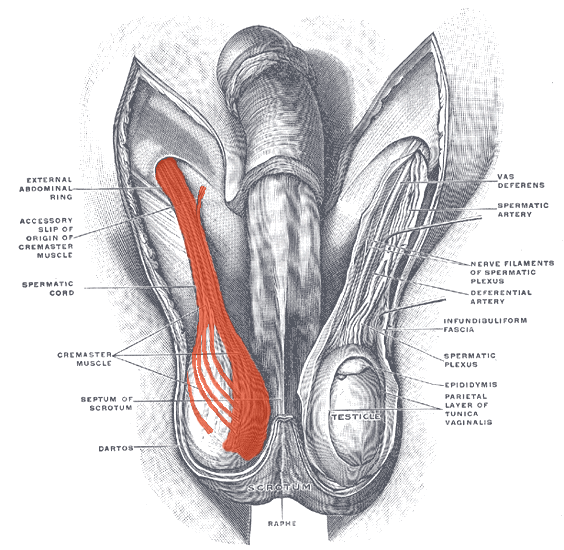
\includegraphics[width=0.5\textwidth]{images/scientiphique/Musculus_cremaster.png}
    \caption{Muscle crémaster}
    \label{fig:muscles-cremaster}
\end{figure}

Ainsi, l'objectif de cette contraception est d'augmenter la température des testicules afin qu'ils ne produisent plus de spermatozoïdes. \cite{wallachRoleTemperatureRegulation1988}
Dans un premier temps l'idée d'utiliser un caleçon avec une résistance chauffante était envisagé et testé. Bien qu'on puisse toujours trouver des exemplaires en vente sur le site suivante : \href{https://www.jemaya-innovations.com/fr/}{https://www.jemaya-innovations.com/fr/}, l'idée n'est pas bonne selon le médecin Roger Mieusset, car le corps va se défendre contre cette source de chaleur extérieure. \cite{guillaumedaudinContraceptesEnqueteDernier2022}

\begin{figure}[h]
    \centering
    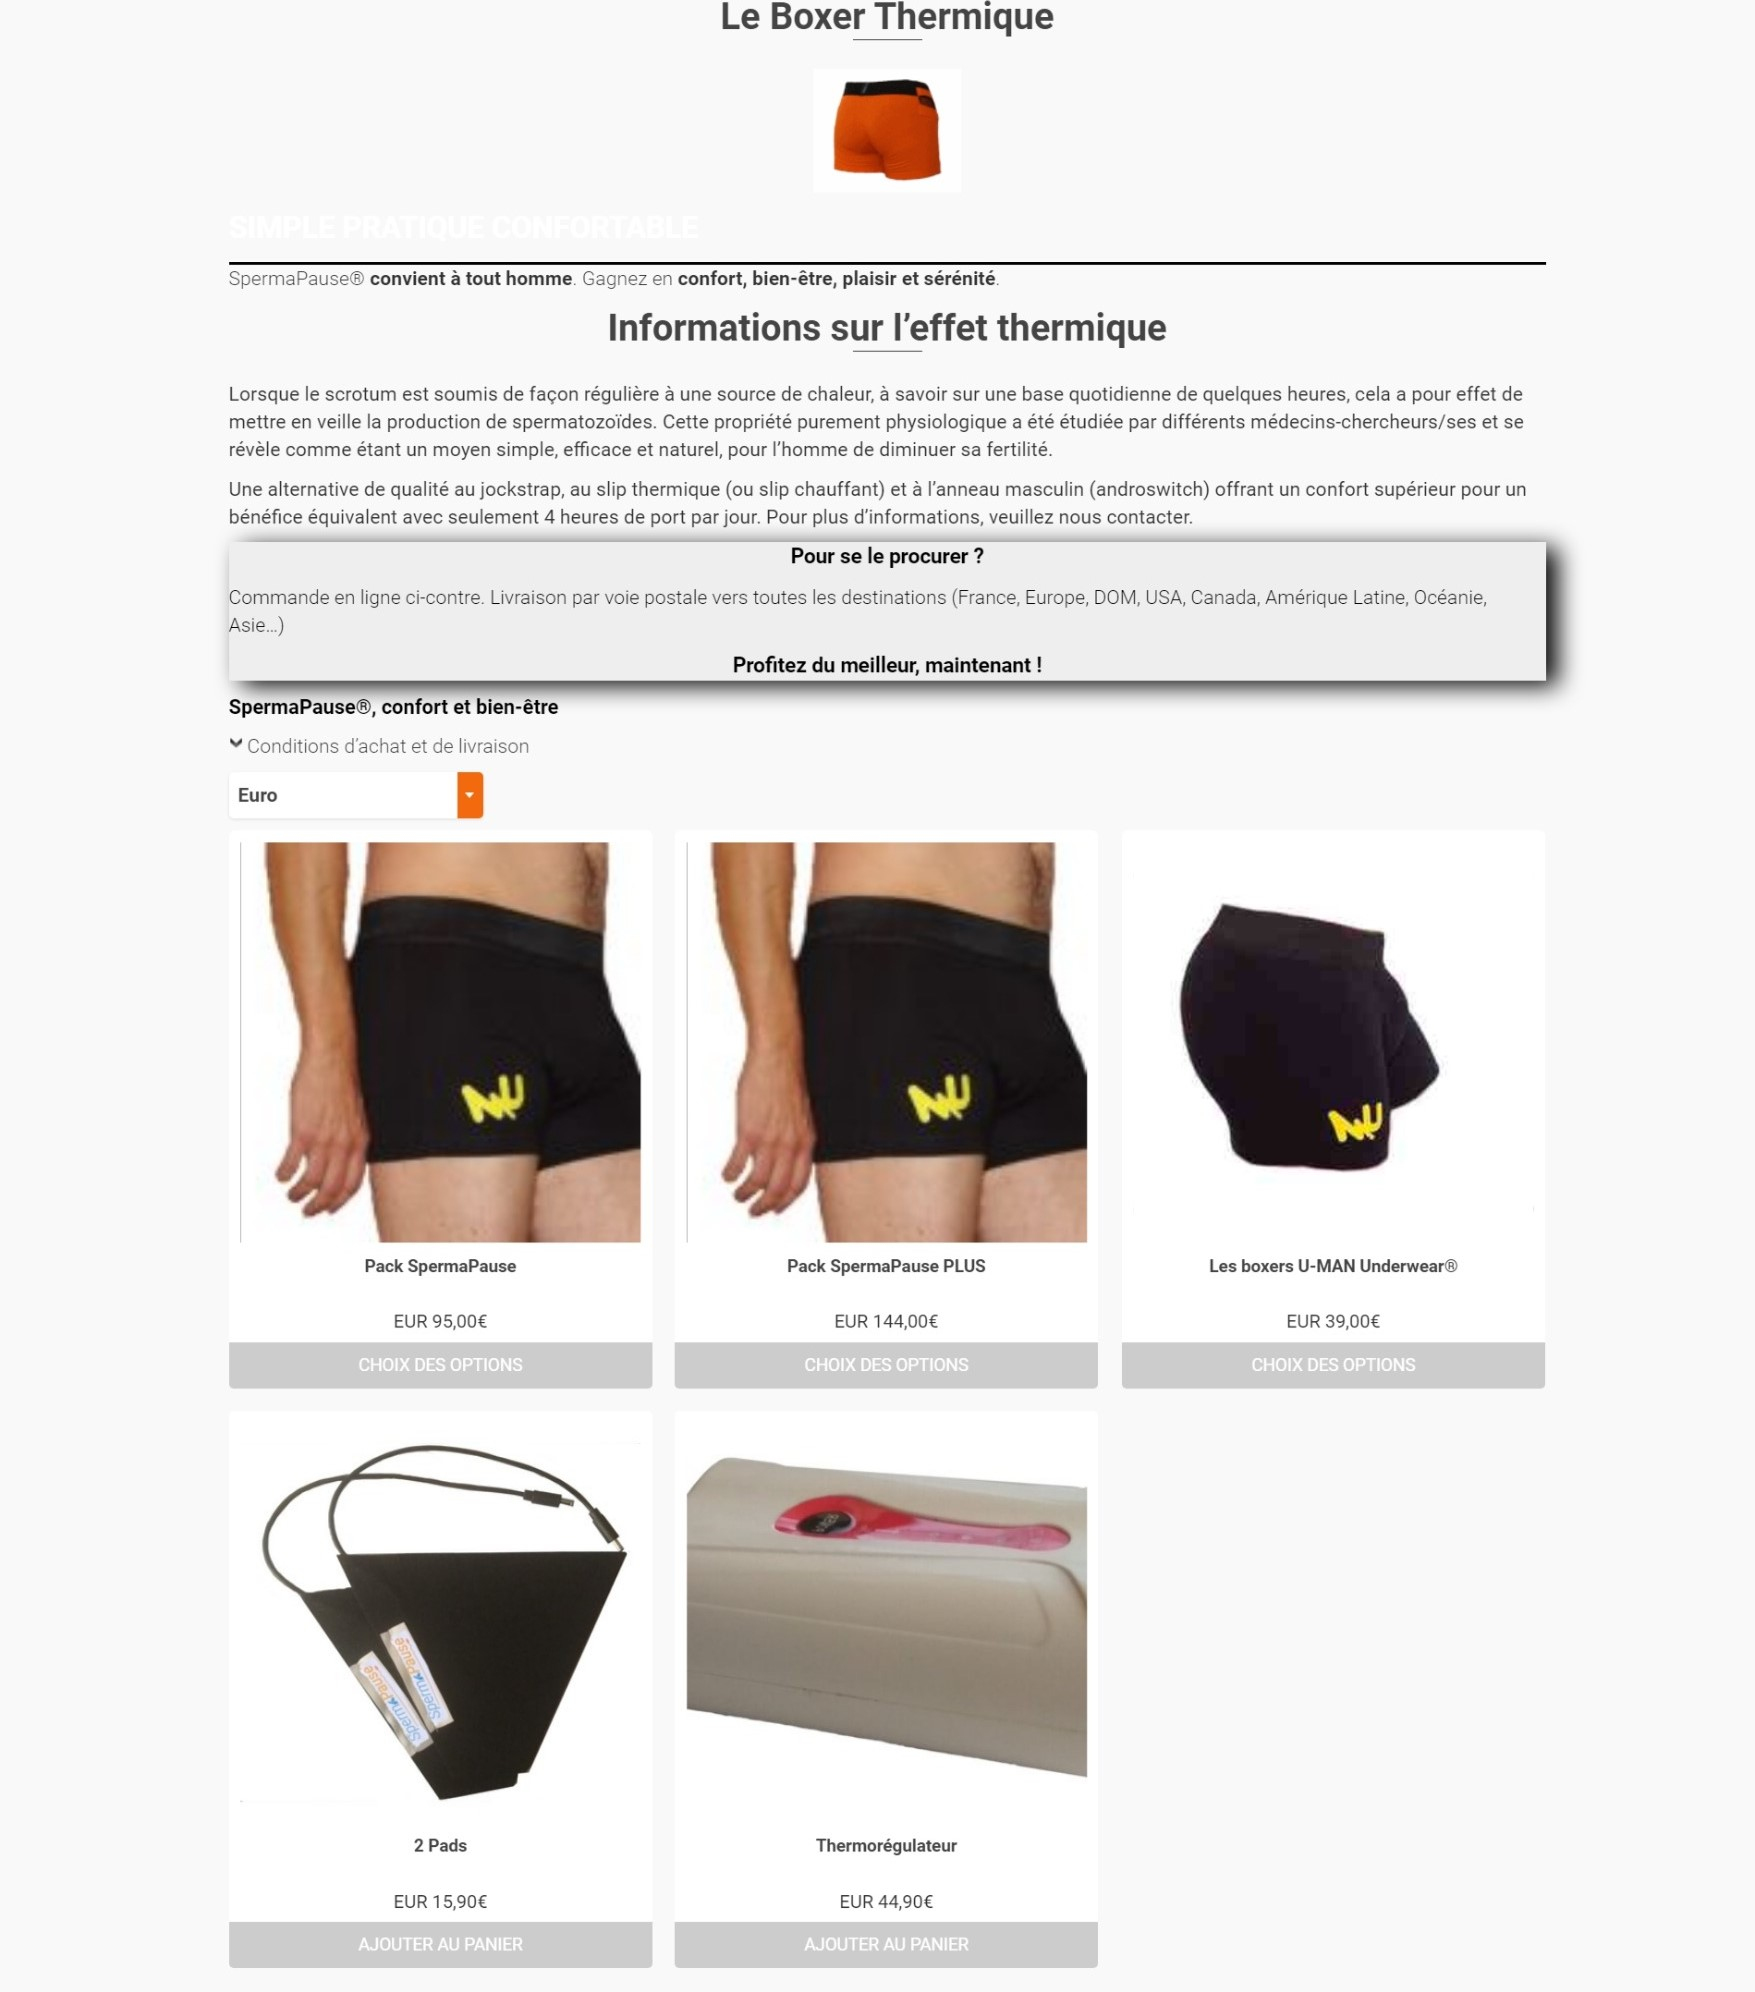
\includegraphics[width=0.6\textwidth]{images/scientiphique/www.jemaya-innovations.com.jpeg}
    \caption{Capture d'écran du site \href{https://www.jemaya-innovations.com/fr/}{https://www.jemaya-innovations.com/fr/} le 18/05/2023}
    \label{fig:site-jemaya}
\end{figure}

L'approche actuelle est donc de réchauffer les testicules en les rapprochant du corps.
Ainsi une étude de 1985 avec 14 volontaires \cite{mieussetInhibitingEffectArtificial1985}, une seconde avec 19 volontaires sur une plus longue période et 1987\cite{mieussetHyperthermiaHumanSpermatogenesis1987}, et une troisième avec 9 volontaires en 1997\cite{mieussetPotentialMildTesticular1994} ont obtenu des résultats concluants.
Cependant, il faut noter que ces 3 études ont comme auteur principal le médecin Roger Mieusset. Ainsi, il faudrait des études complémentaires menées par d'autres scientifiques.

On se rend compte que cette méthode qui vise à rapprocher les testicules du corps, est très proche d'une Cryptorchidie.
Selon Wikipédia: <<La cryptorchidie, appelée aussi trouble de la migration du testicule, ou plus communément testicule mal descendu, est l'absence d'un ou des deux testicules dans le scrotum (position normale introscrotale chez l'homme et chez les animaux à testicules externes).>>\cite{Cryptorchidie2023a}

\begin{figure}[H]
    \centering
    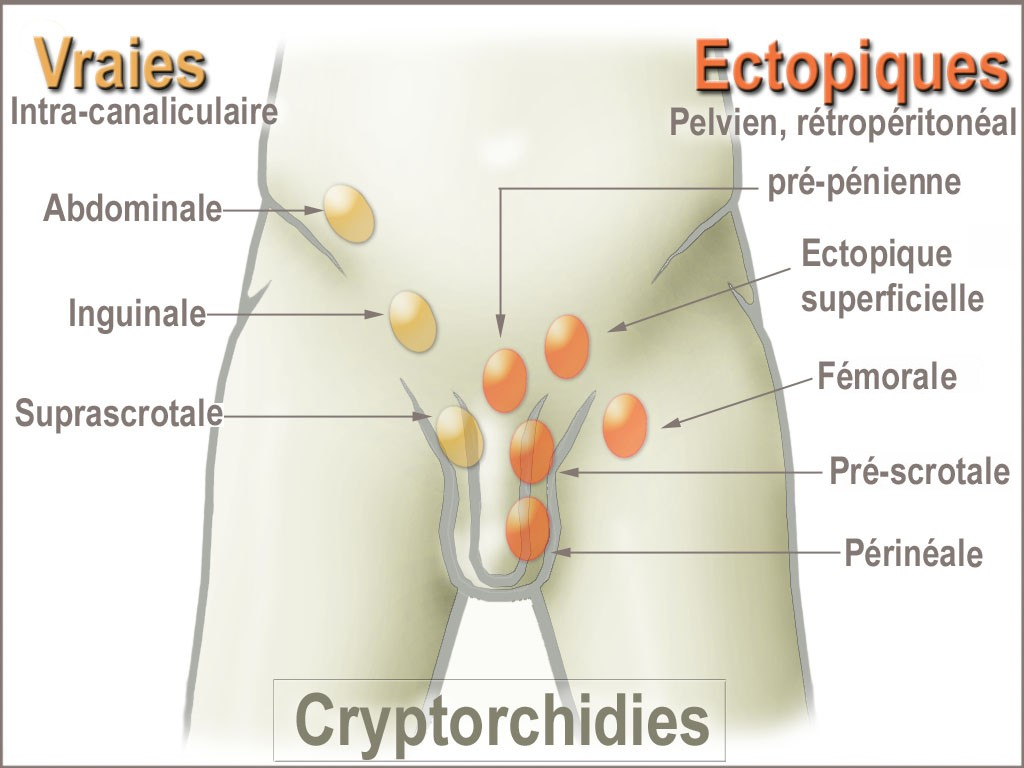
\includegraphics[width=0.4\textwidth]{images/scientiphique/CryptorchidismForms.jpg}
    \caption{Cryptorchidie par Lamiot — Travail personnel, CC BY-SA 3.0, \href{https://commons.wikimedia.org/w/index.php?curid=9736634}{https://commons.wikimedia.org/w/index.php?curid=9736634}}
    \label{fig:cryptorchidie}
\end{figure}

Il est connu que la cryptorchidie augmente le risque de cancer testiculaire. \cite{CryptorchidieOuTesticule}
Ainsi, il faudrait faire des études complémentaires pour vérifier si cette méthode de contraception augmente aussi le cancer du testicule, en particulier sur le long terme. De plus, la réversibilité de la méthode n'a jamais été testé pour plus de 4 ans. \cite{NoticeUtilisationPdf2022}

Cependant, malgré que ni l'OMS, ni le ministère de la Santé reconnaissent cette méthode, elle a été jugée fiable et sans effets secondaires par Association française d'urologie.\cite{ContraceptionMasculineAucune2021}
De plus on peut retrouver de multiples témoignages de personnes qui l'utilisent avec succès.
Parmi ces témoignages on pout citer Guillaume Daudin, journaliste à l'agence France-Presse qui a écrit un livre sur la contraception masculine. \cite{guillaumedaudinContraceptesEnqueteDernier2022}
On peut donc considérer que ce témoignage est fiable et qu'il ne s'agit pas d'un canular.

Ainsi, aujourd'hui, les deux méthodes pour rapprocher les testicules sont les suivantes :
\begin{itemize}
    \item L'anneau contraceptif
    \item Le slip chauffant. Attention, il ne s'agit pas du caleçon chauffant évoqué précédemment avec une résistance.
\end{itemize}

Une fois mis en place, il doit être porté 15 heures par jour. Comme la méthode hormonale, il faut attendre 3 mois avant que la méthode de contraception soit efficace. \cite{anne-sophiedelcourHommeSousPilule}
De plus, afin d'être sûr que la personne est stérile, on effectue un spermogramme avant de commencer et un autre 3 mois après. \cite{MethodeThermique}

\subsubsection{Le slip chauffant}

Le slip chauffant se présente sous la forme d'un slip avec un trou en forme d'anneau permettant de faire passer la verge et les poches des testicules tout en maintenant les testicules au niveau du corps. \cite{MethodeThermique}

\begin{figure}[h]
    \centering
    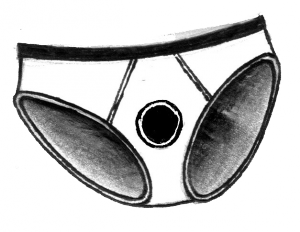
\includegraphics[width=0.3\textwidth]{images/scientiphique/slip_chauffant.png}
    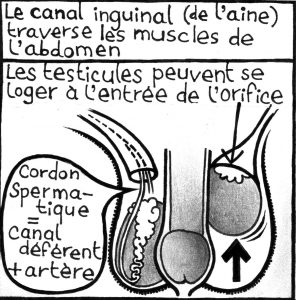
\includegraphics[width=0.3\textwidth]{images/scientiphique/slip_chauffant_mise_en_place_1.png}
    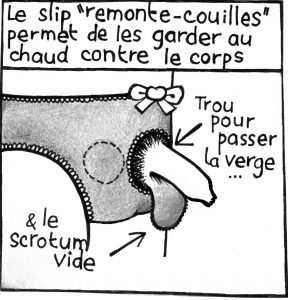
\includegraphics[width=0.3\textwidth]{images/scientiphique/slip_chauffant_mise_en_place_2.png}
    \caption{Illustration de la mise en place du slip chauffant par l'ARDECOM \cite{MethodeThermique}}
    \label{fig:slip_chauffant}
\end{figure}

Ces slips sont majoritairement fabriqués par les personnes elles-mêmes. Ceci permet d'éviter les problèmes liés à la vente d'une méthode de contraception qui n'a pas été validé par la Haute Autorité de Santé. \cites{MethodeThermique}{guillaumedaudinContraceptesEnqueteDernier2022}
Il existe des ateliers pour apprendre à confectionner ces slips avec le matériel nécessaire mis à disposition. \cites{ContraceptionMasculineComment2023}{guillaumedaudinContraceptesEnqueteDernier2022}
De plus on peut trouver des tutoriels en lignes pour apprendre à les fabriquer.

\begin{figure}[H]
    \centering
    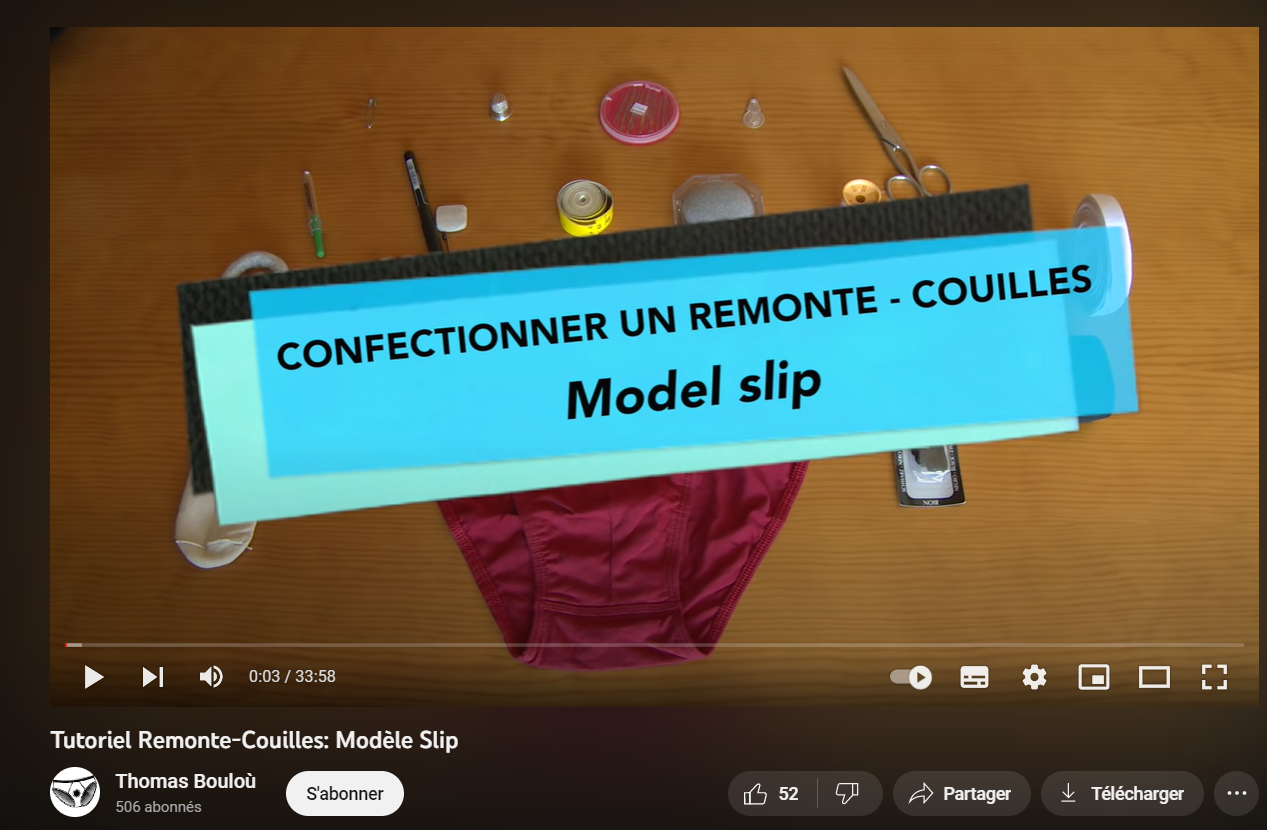
\includegraphics[width=0.5\textwidth]{images/scientiphique/Tuto_slip_contraceptif.png}
    \caption{Exemple de tutoriel pour fabriquer un slip chauffant disponible à l'adresse suivante : \href{https://www.youtube.com/watch?v=AjZBcK4WzI8}{https://www.youtube.com/watch?v=AjZBcK4WzI8}}
    \label{fig:tuto_slip_chauffant}
\end{figure}

\subsubsection{L'anneau contraceptif}

Le concept de l'anneau contraceptif est le même que celui du slip chauffant, à la différence qu'il s'agit d'un anneau en silicone qui se place à la base du pénis et peut ainsi tenir tout seul.

\begin{figure}[h]
    \centering
    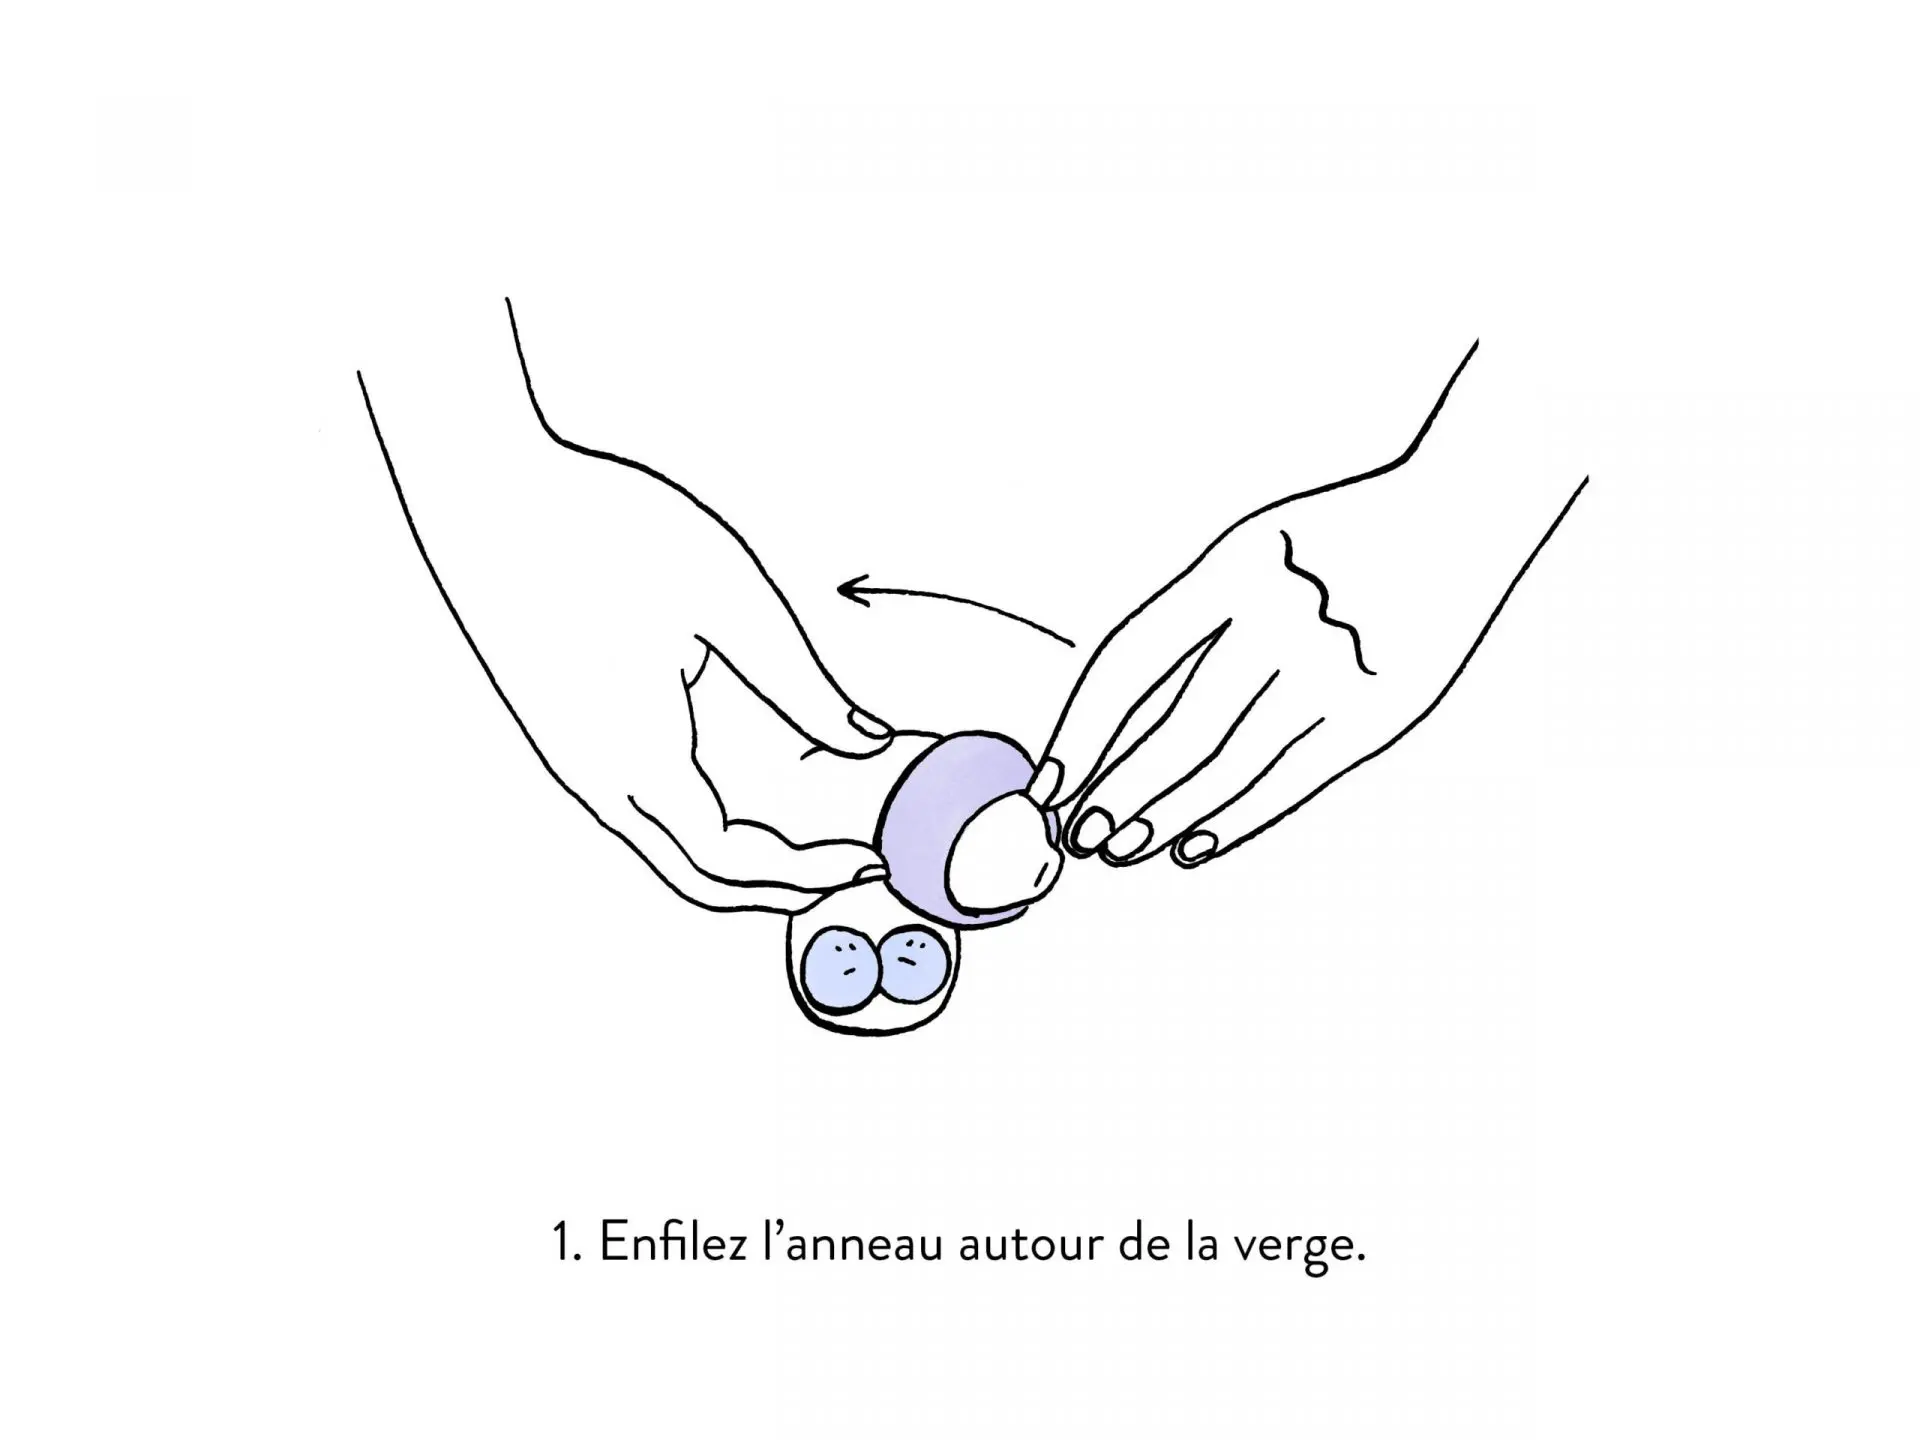
\includegraphics[width=0.3\textwidth]{images/scientiphique/Tuto_andro_switch/1.png}
    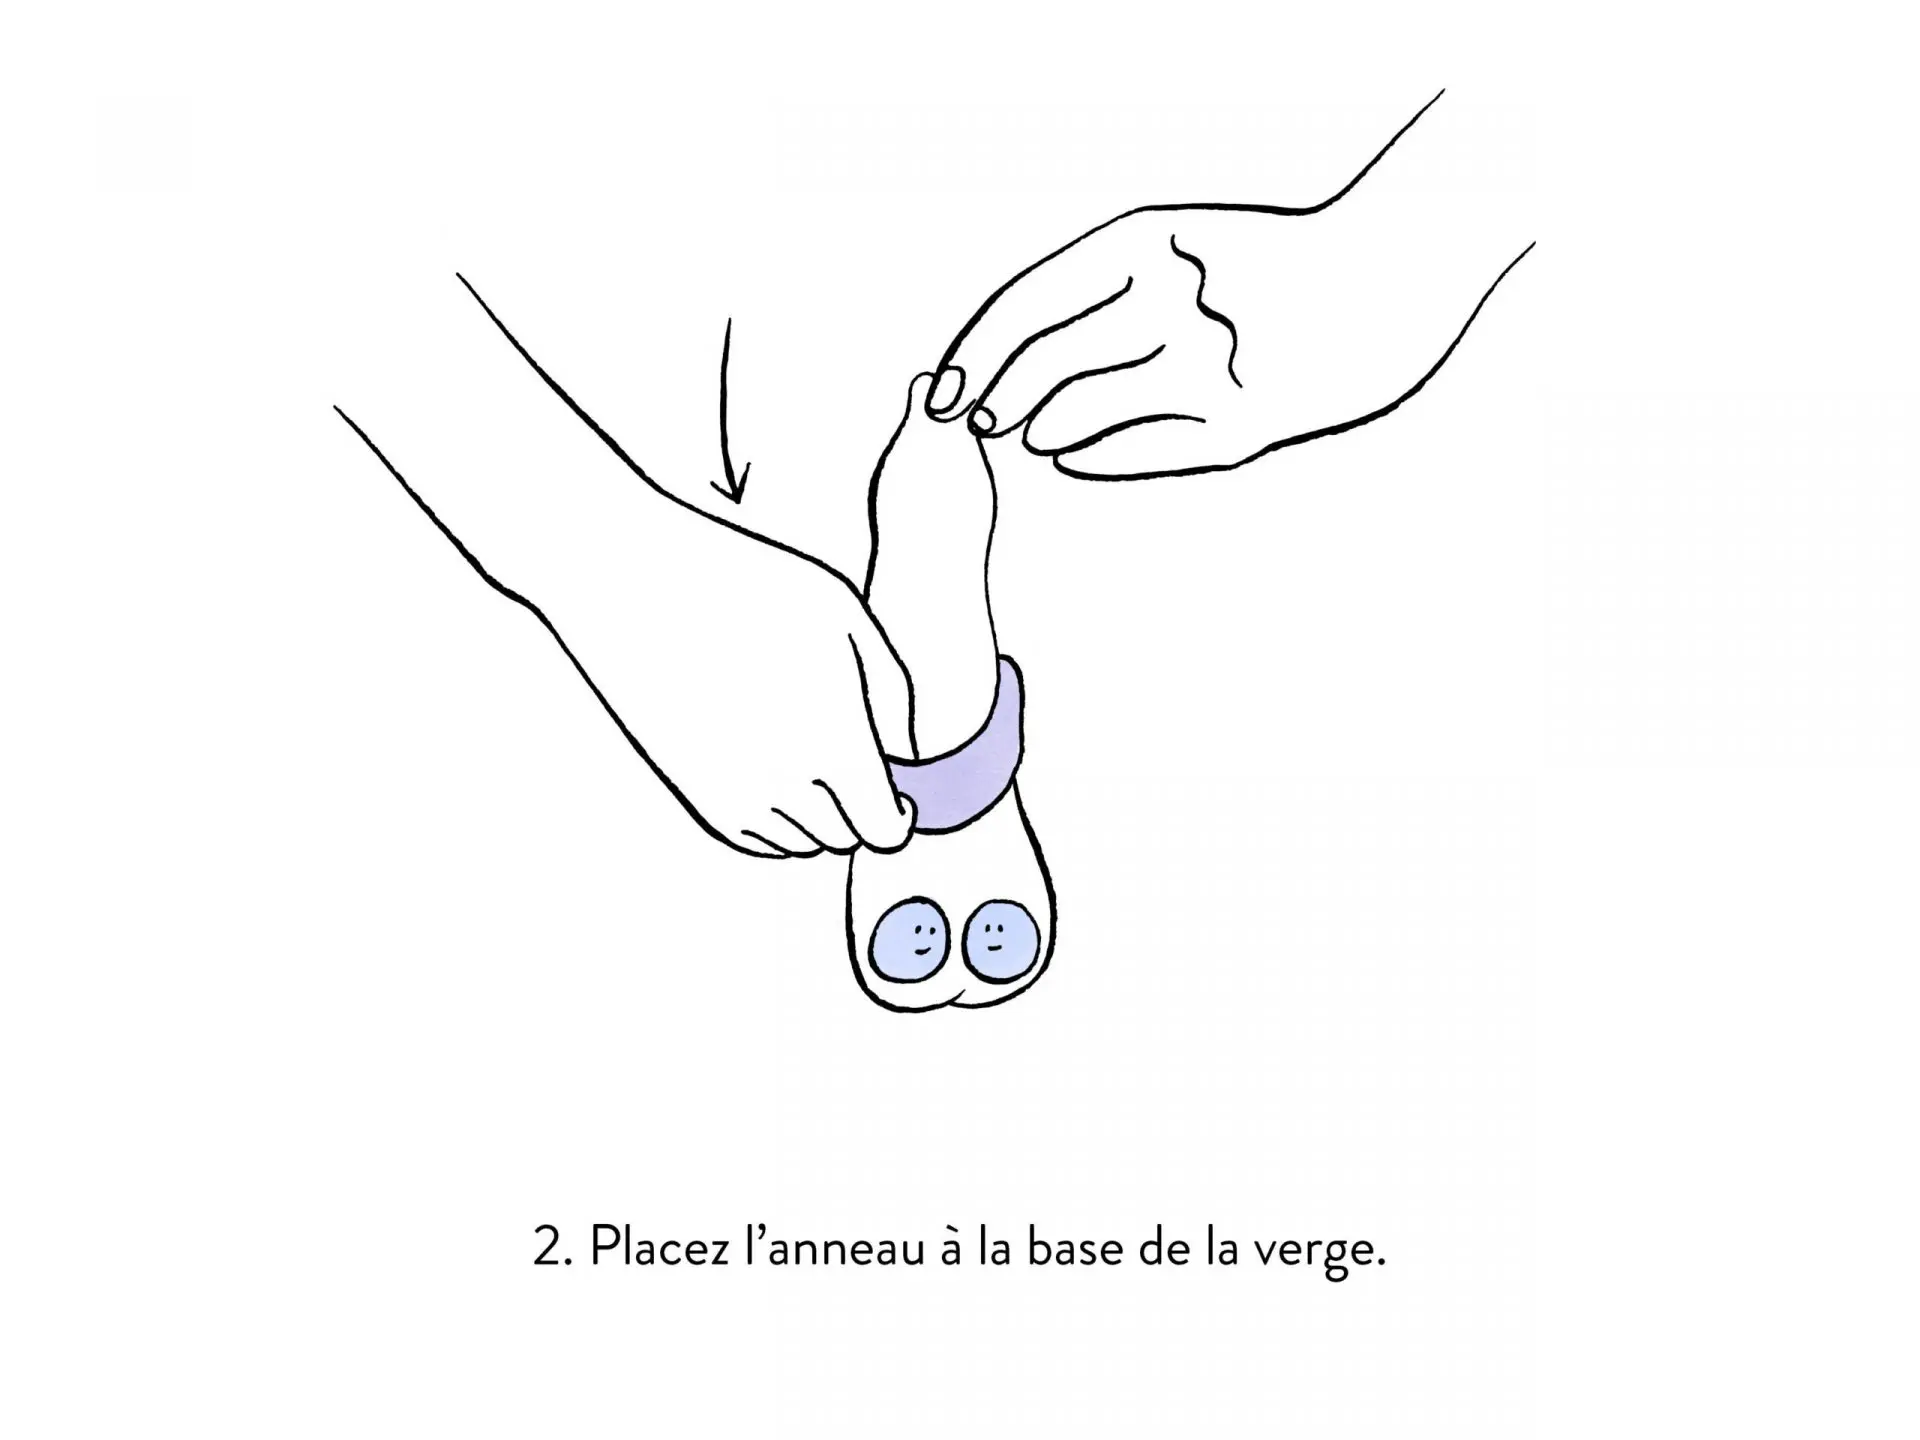
\includegraphics[width=0.3\textwidth]{images/scientiphique/Tuto_andro_switch/2.png}
    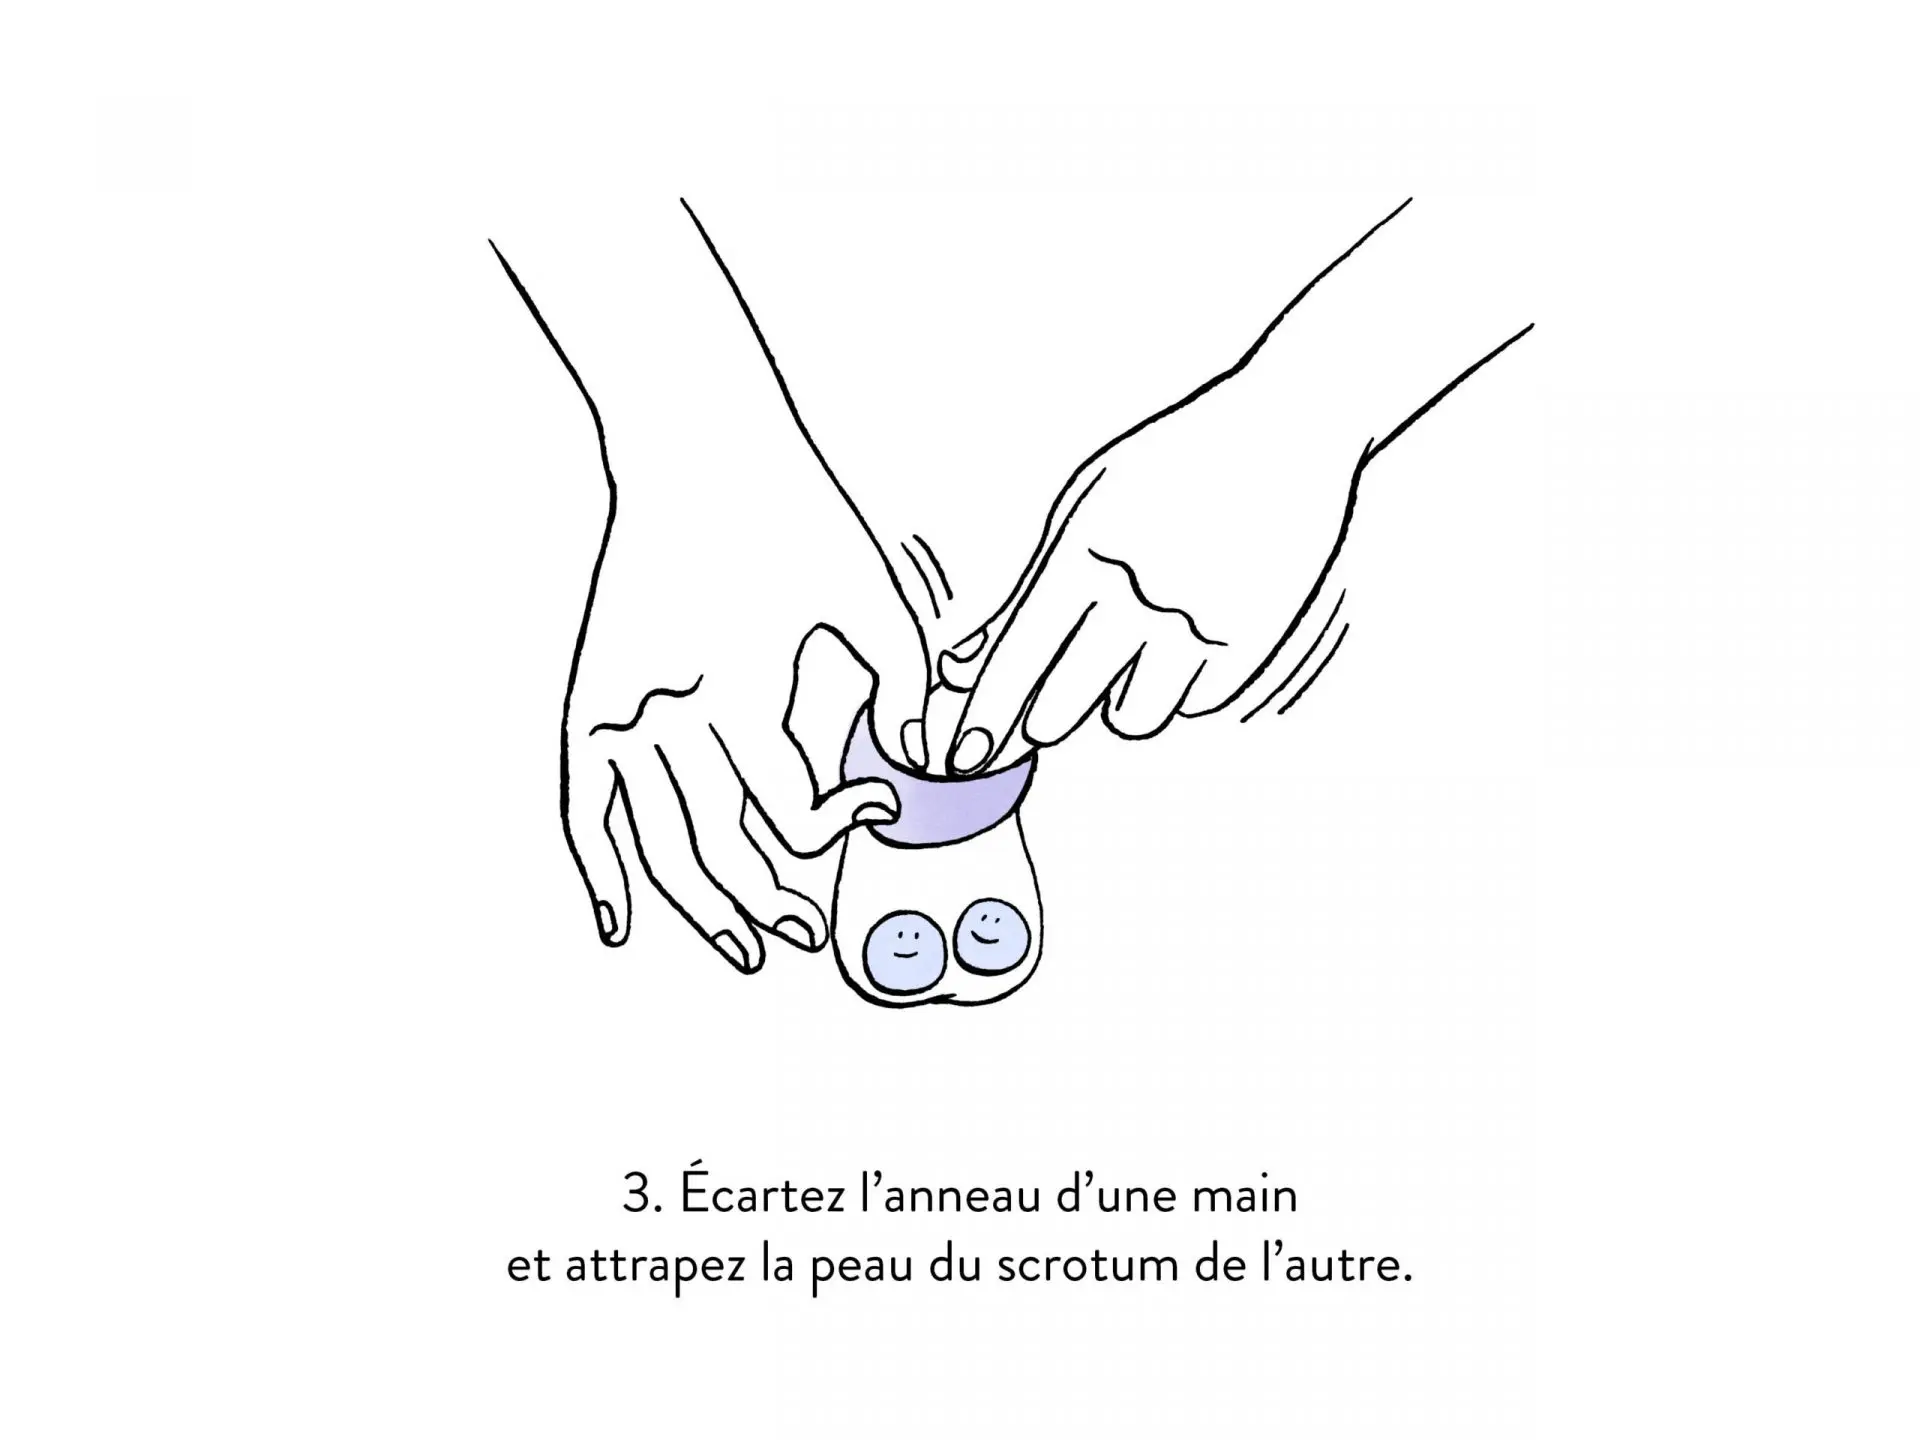
\includegraphics[width=0.3\textwidth]{images/scientiphique/Tuto_andro_switch/3.png}
    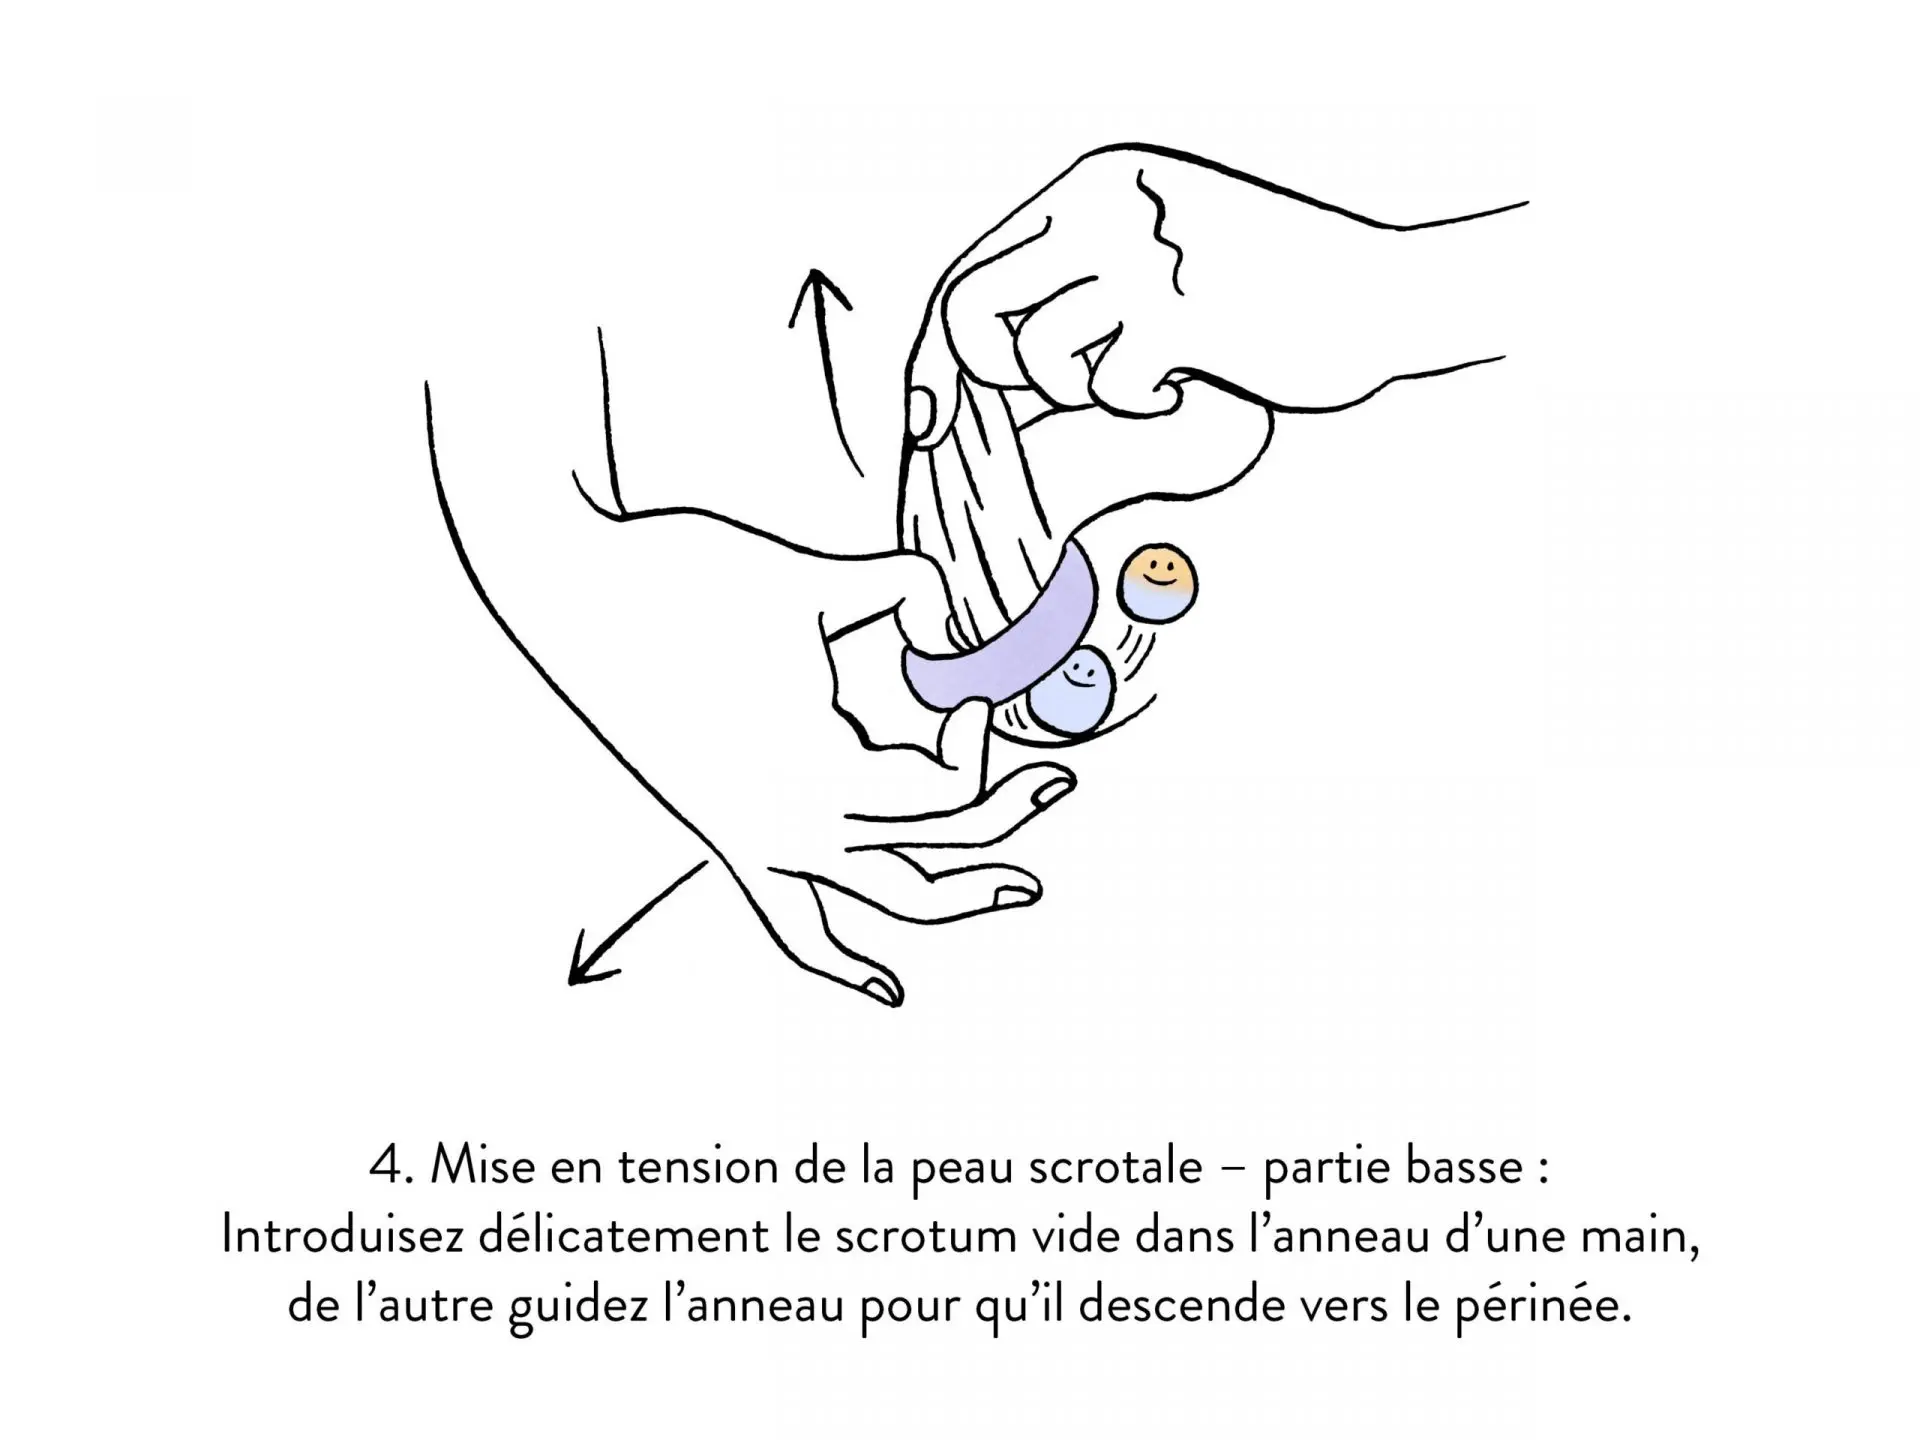
\includegraphics[width=0.3\textwidth]{images/scientiphique/Tuto_andro_switch/4.png}
    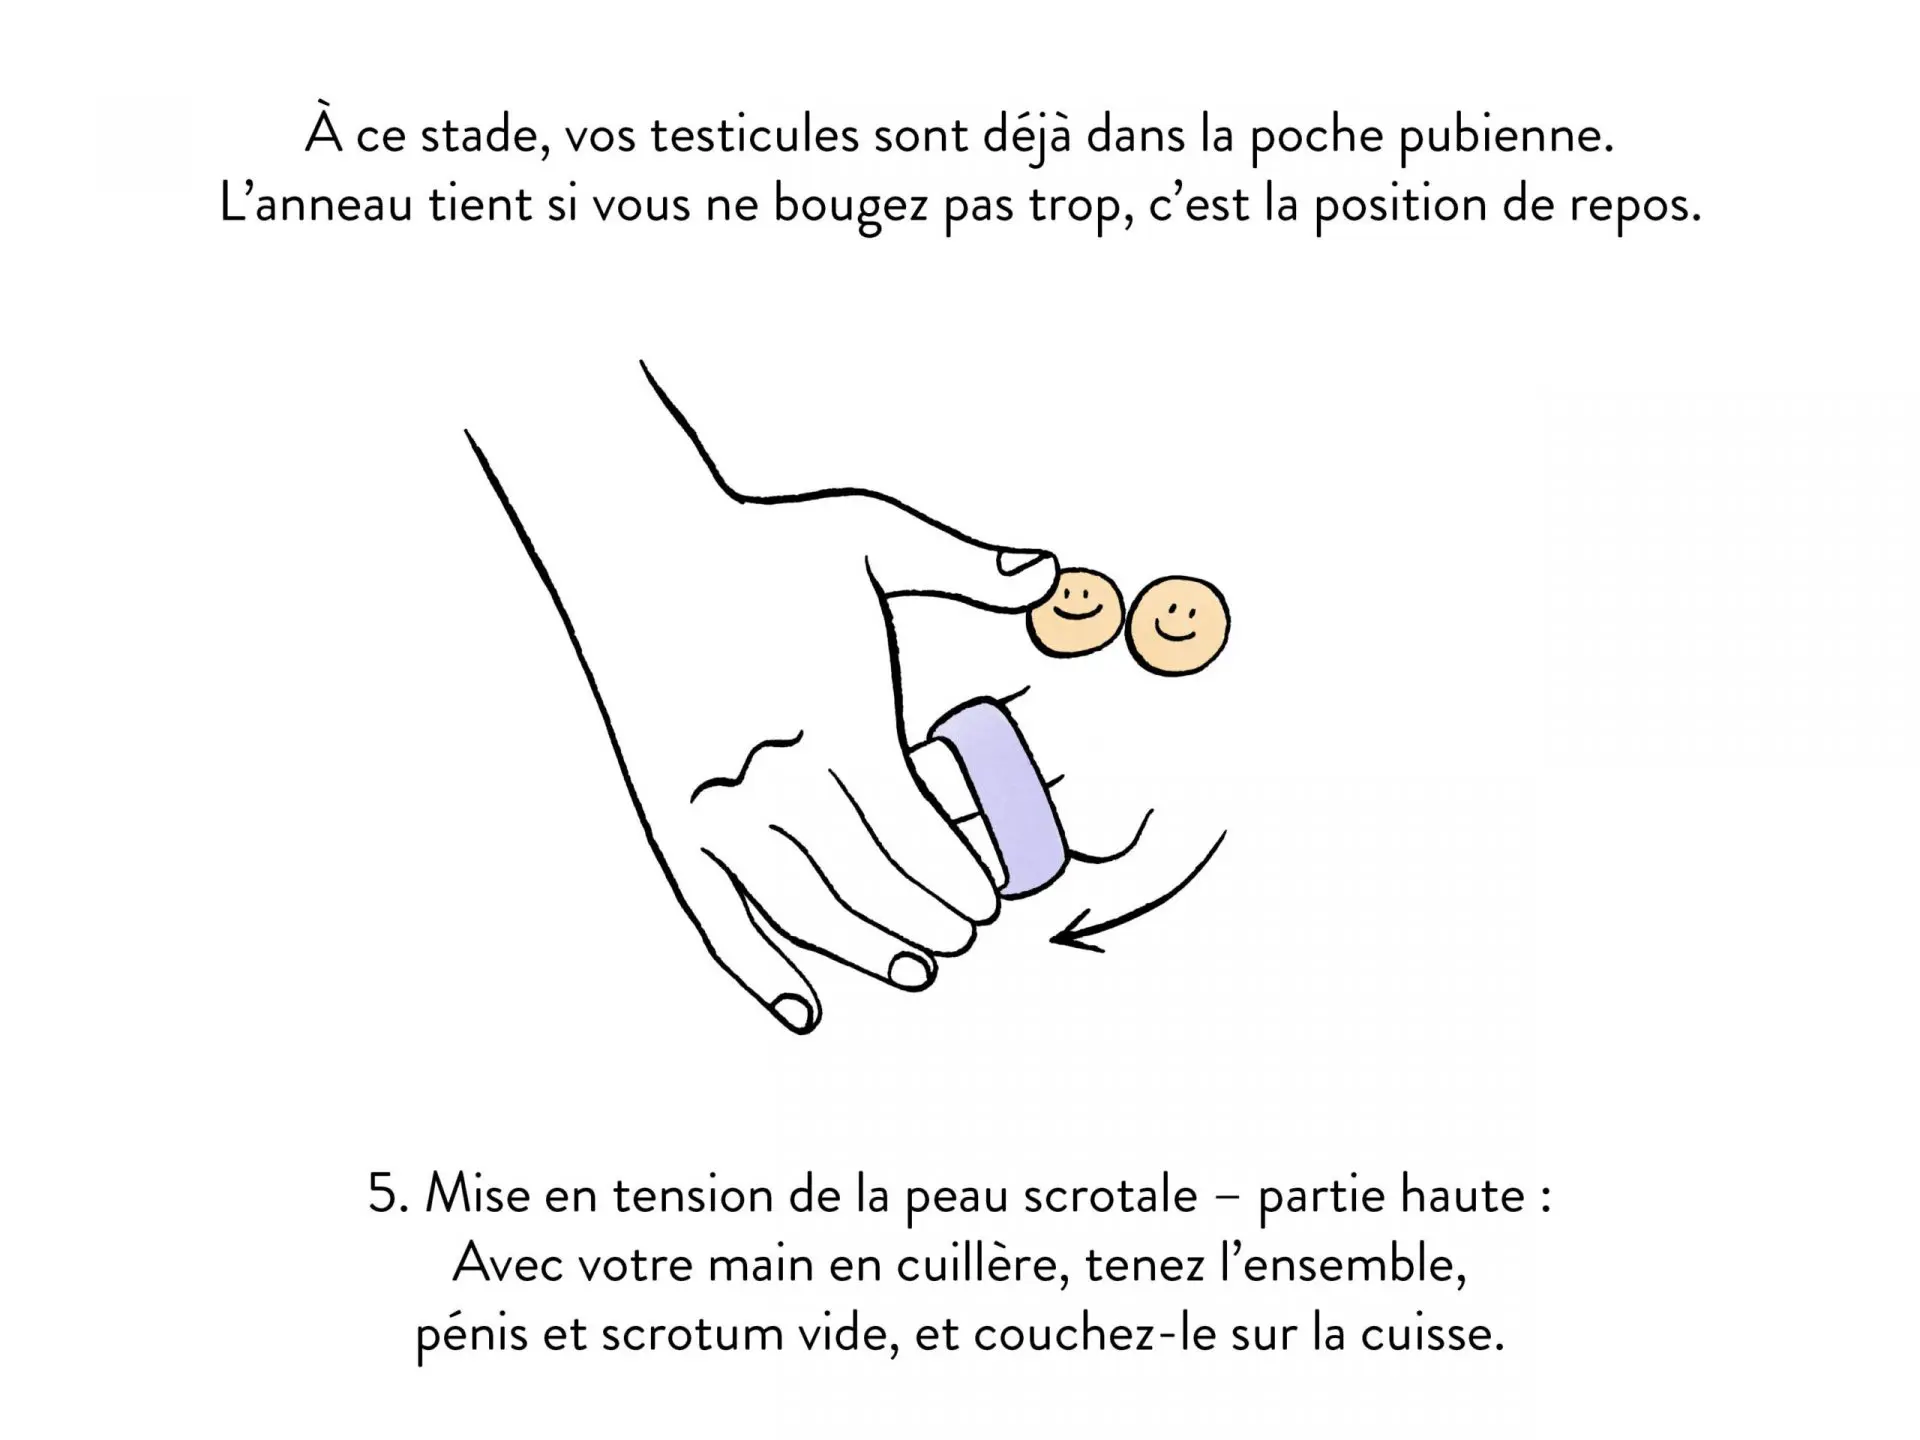
\includegraphics[width=0.3\textwidth]{images/scientiphique/Tuto_andro_switch/5.png}
    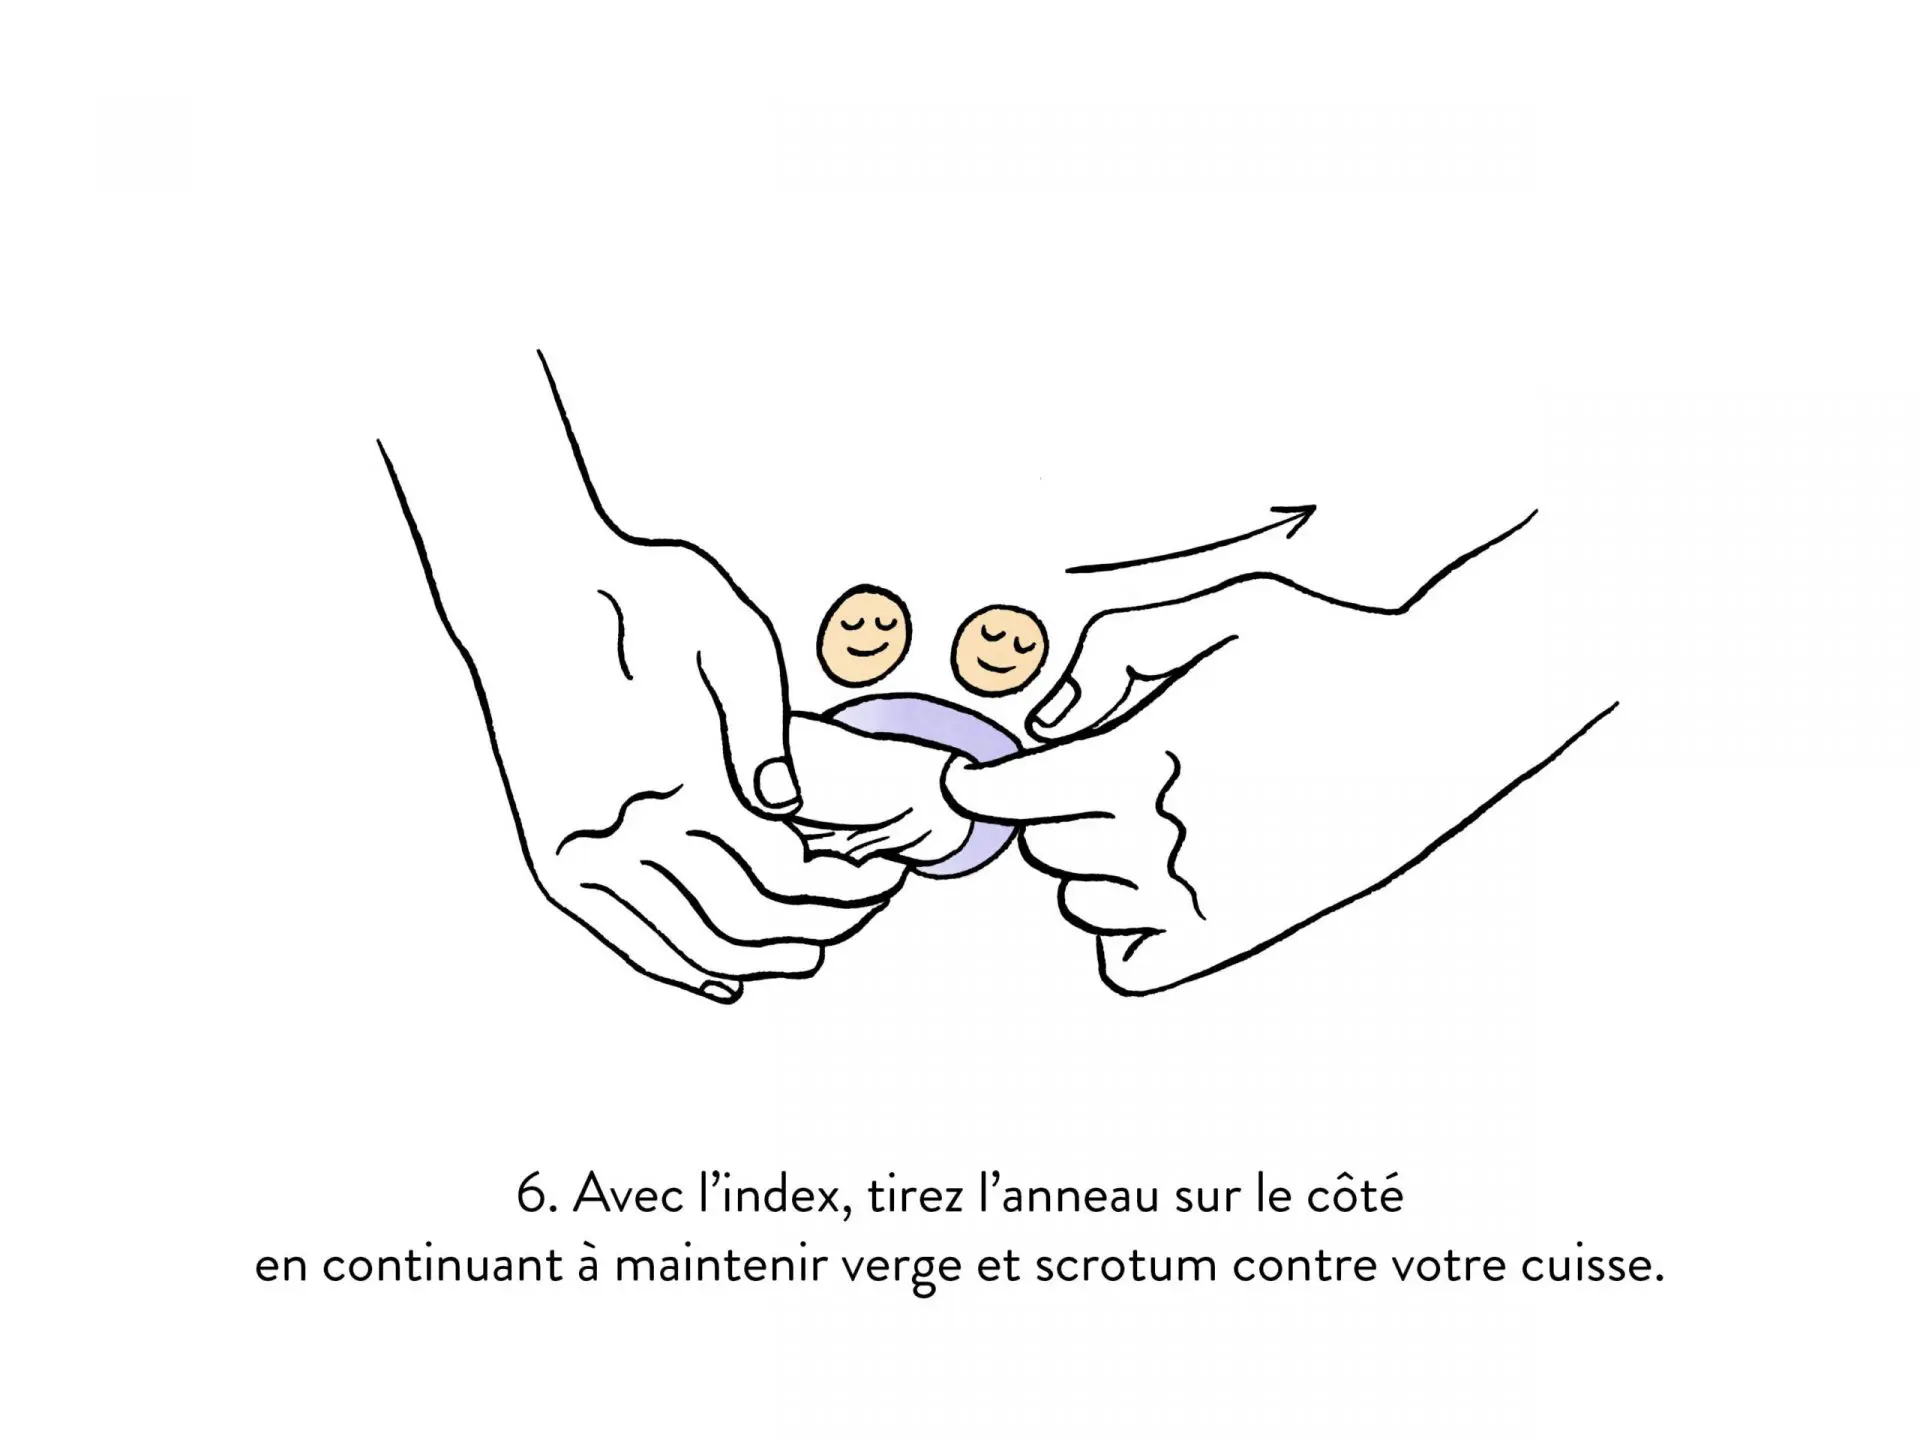
\includegraphics[width=0.3\textwidth]{images/scientiphique/Tuto_andro_switch/6.png}
    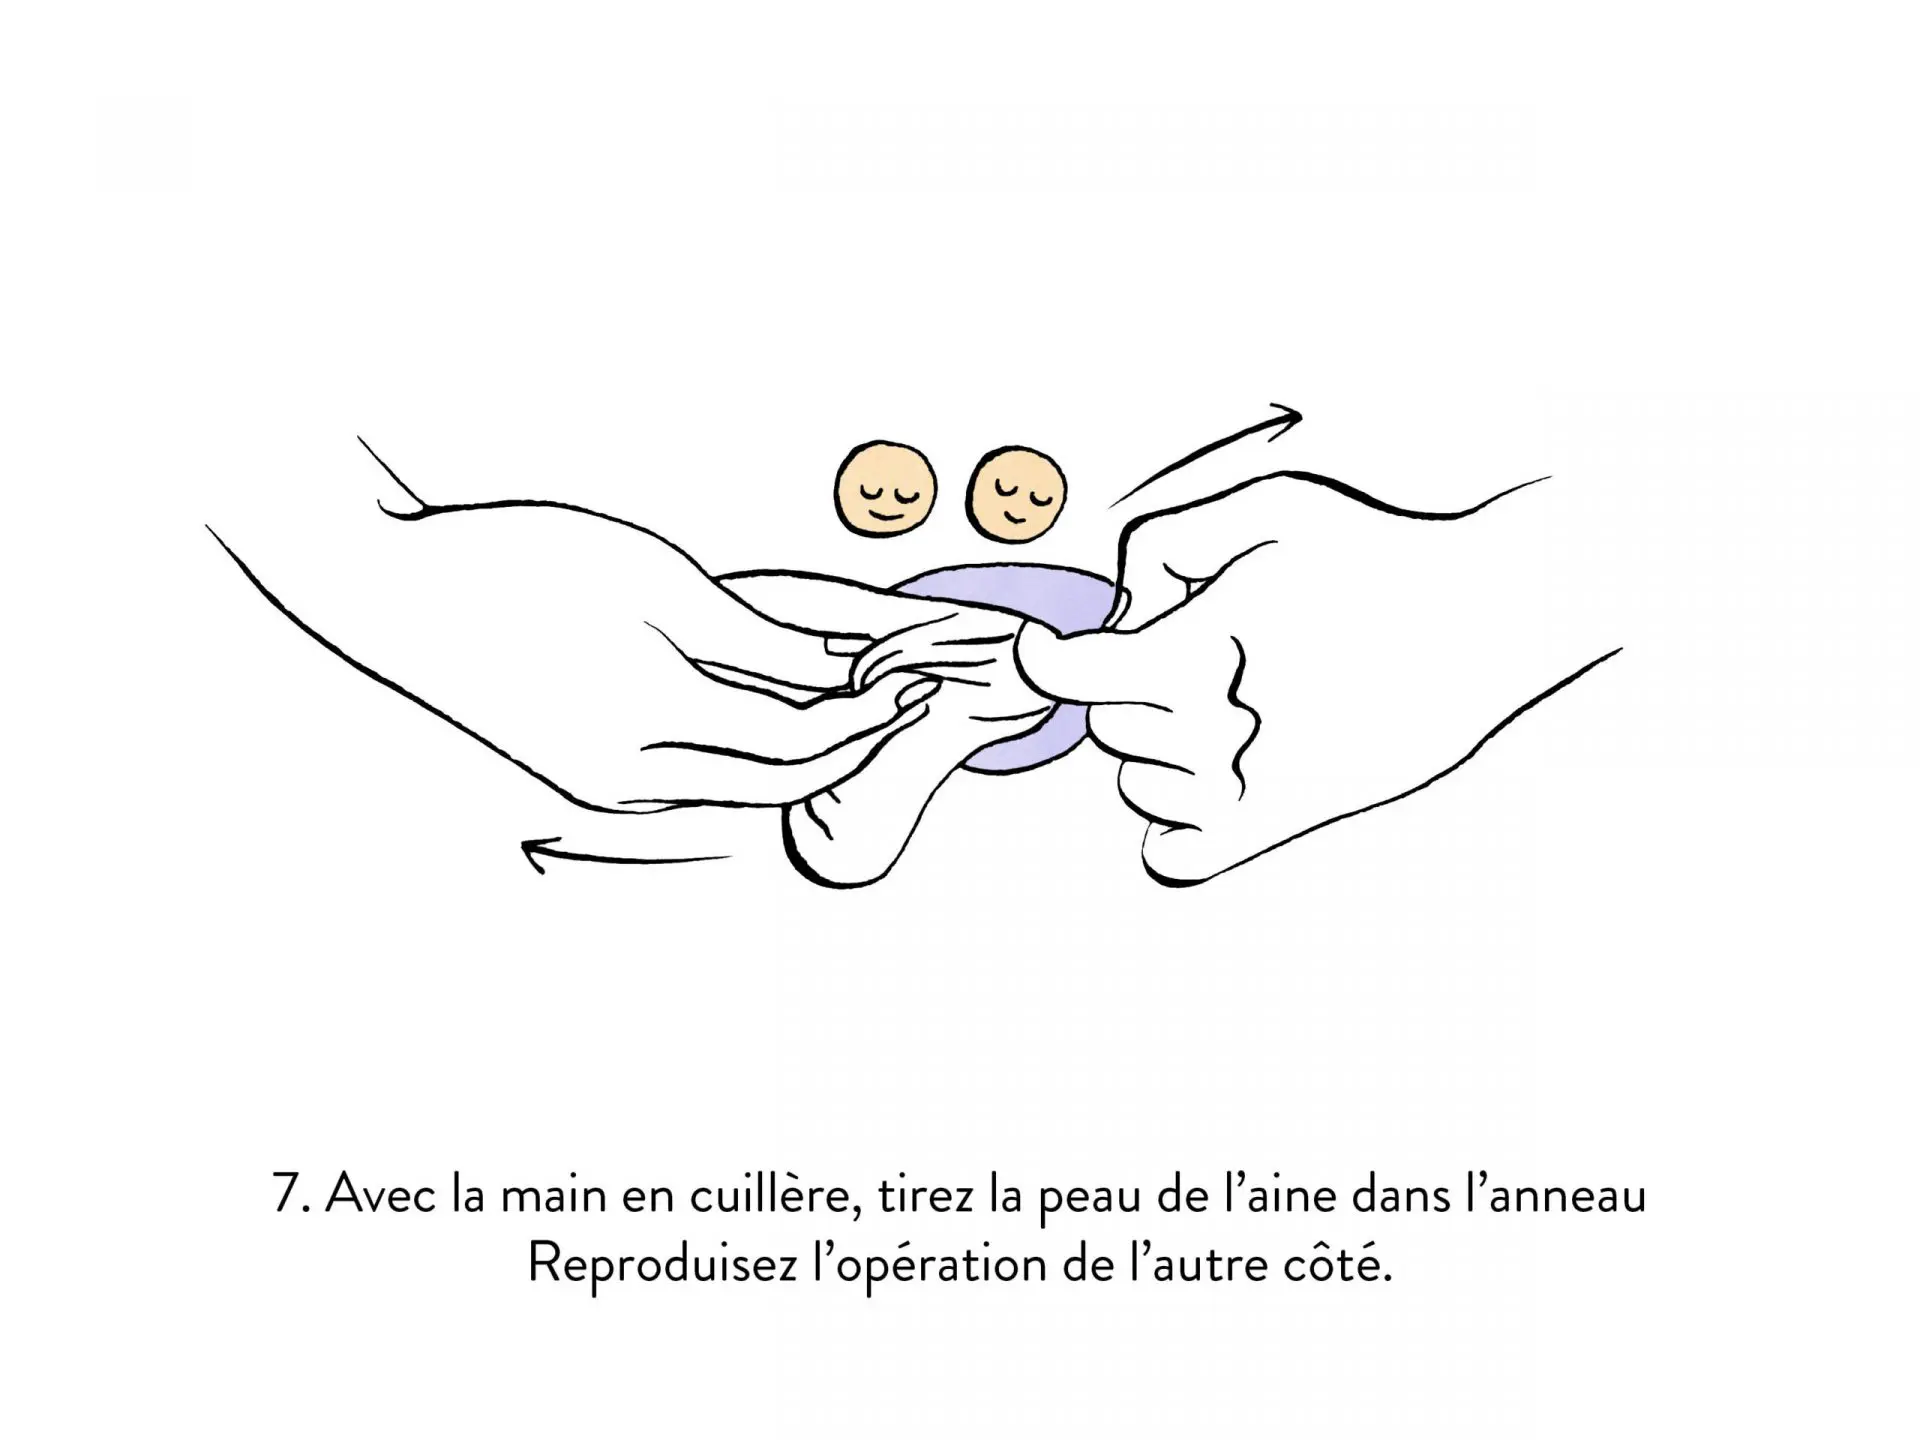
\includegraphics[width=0.3\textwidth]{images/scientiphique/Tuto_andro_switch/7.png}
    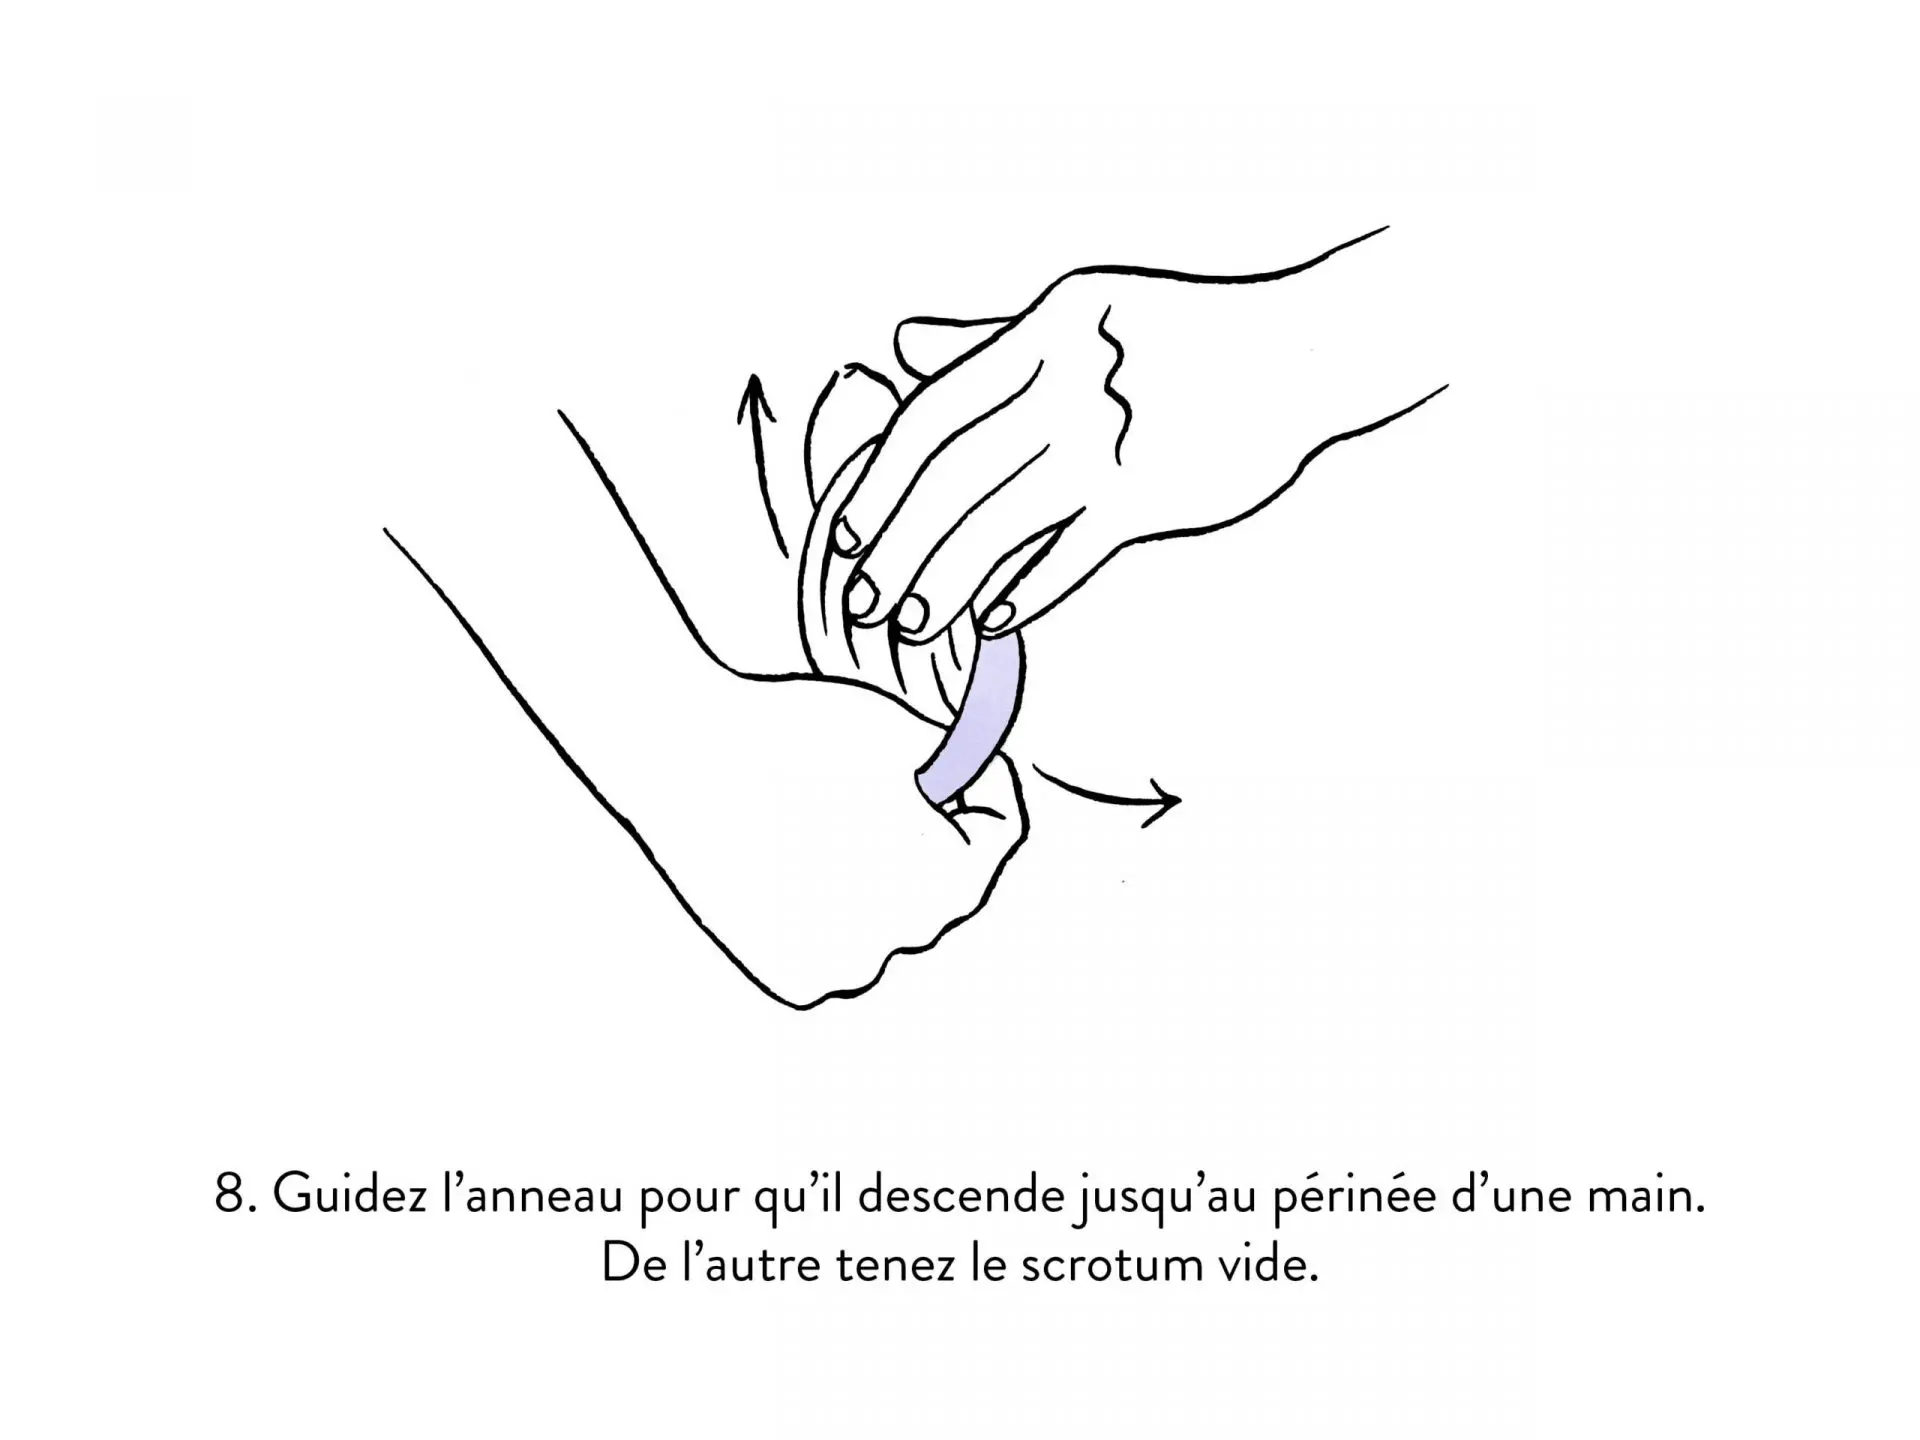
\includegraphics[width=0.3\textwidth]{images/scientiphique/Tuto_andro_switch/8.png}
    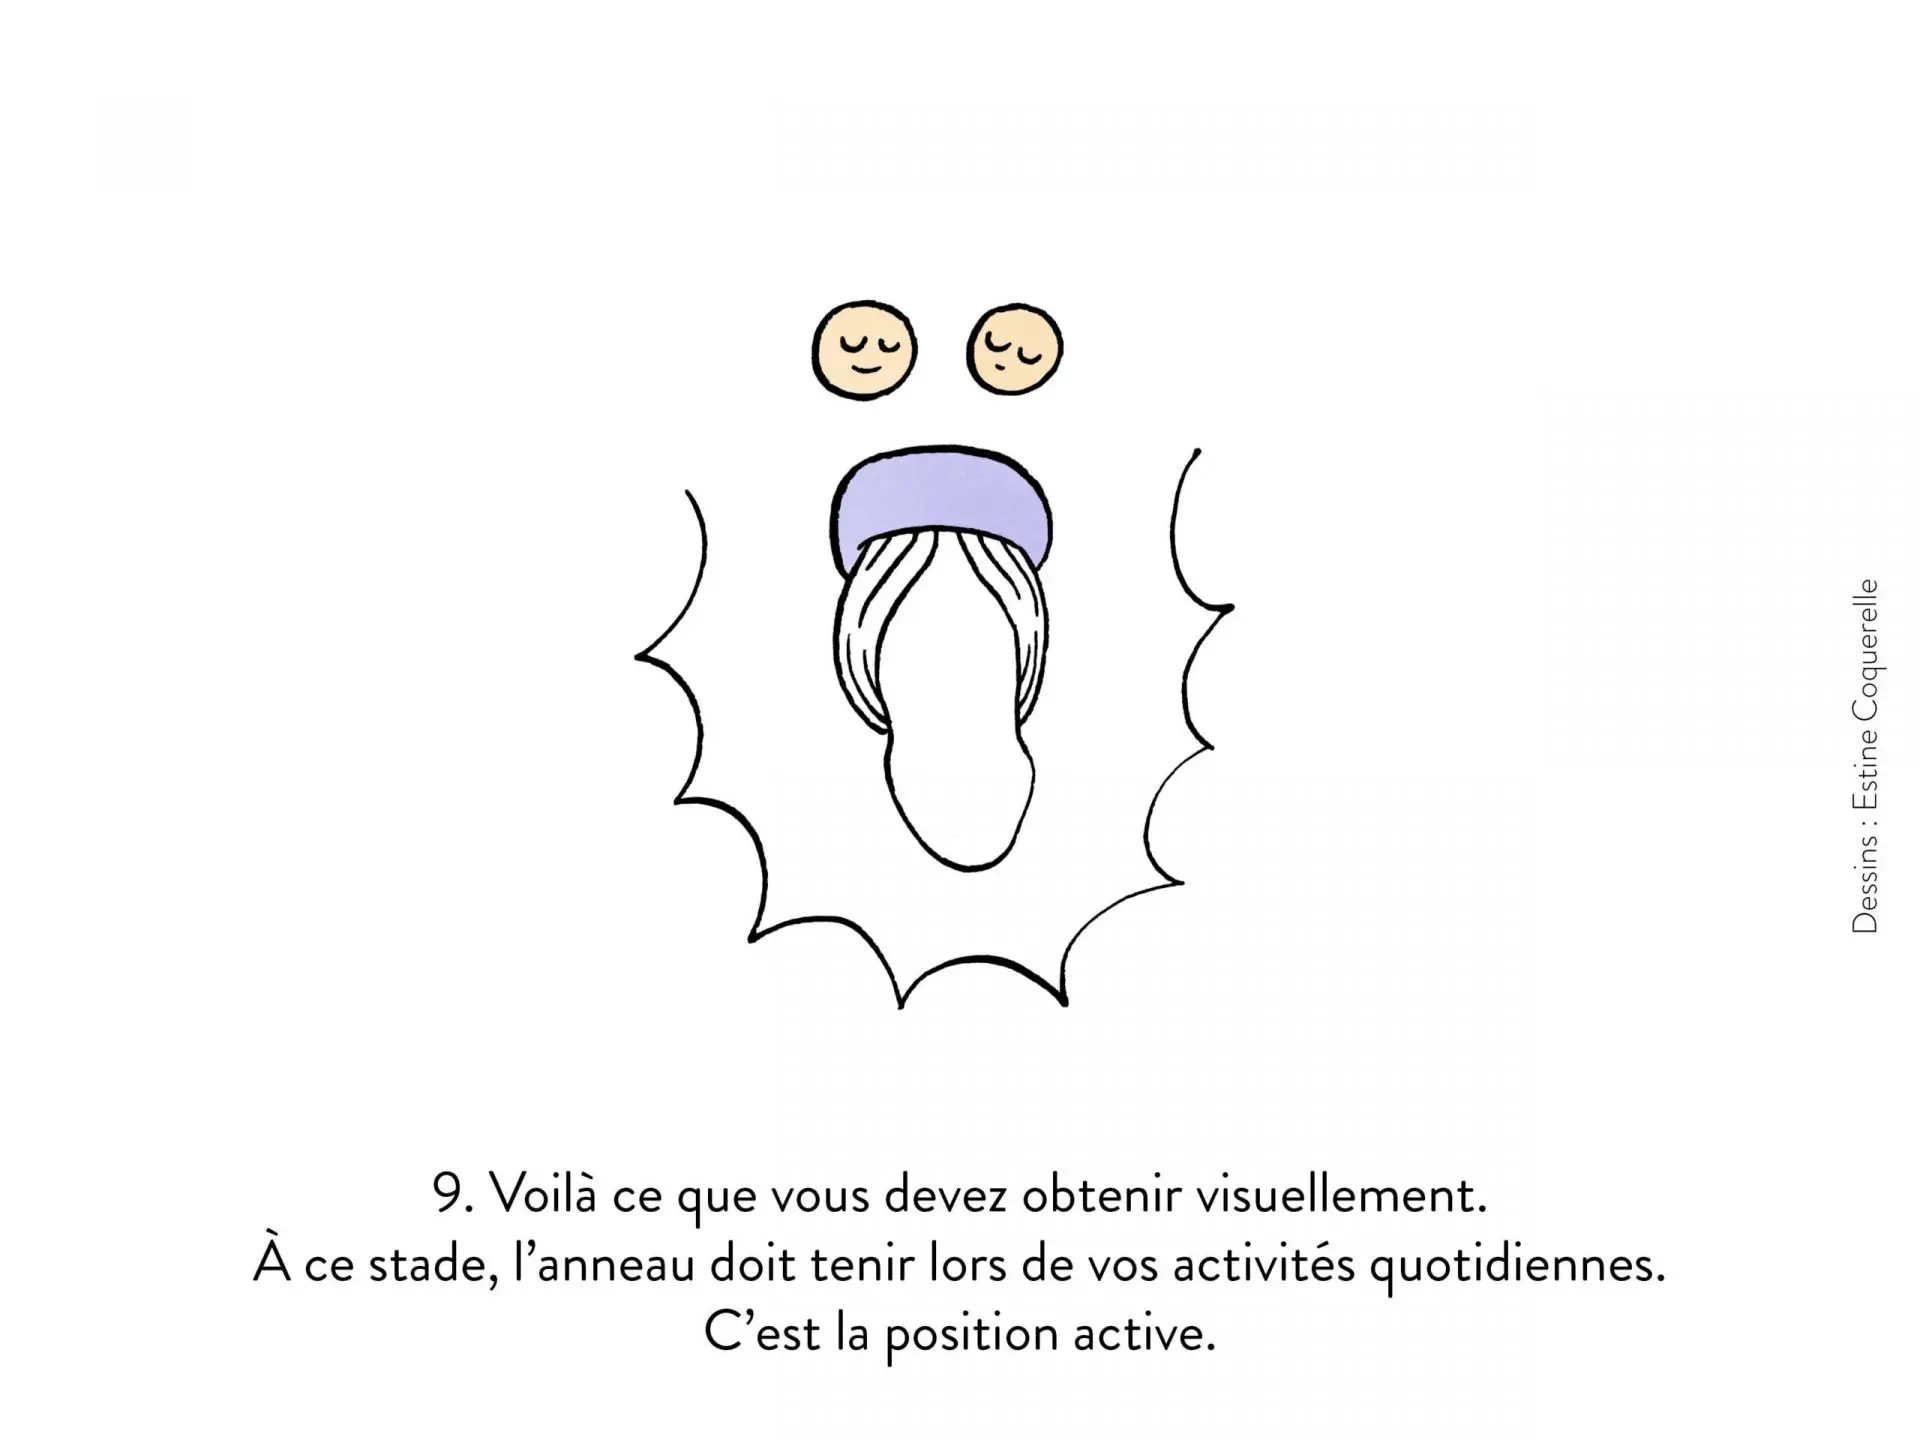
\includegraphics[width=0.3\textwidth]{images/scientiphique/Tuto_andro_switch/9.png}
    \caption{Tutoriel pour mettre en place l'anneau contraceptif par THOREME}
    \label{fig:tuto_andro_switch}
\end{figure}

En France Maxime Labrit via sa société Thoreme commercialisait cet anneau sous le nom d'\textit{Andro-Switch}. \cite{guillaumedaudinContraceptesEnqueteDernier2022}

\begin{figure}[H]
    \centering
    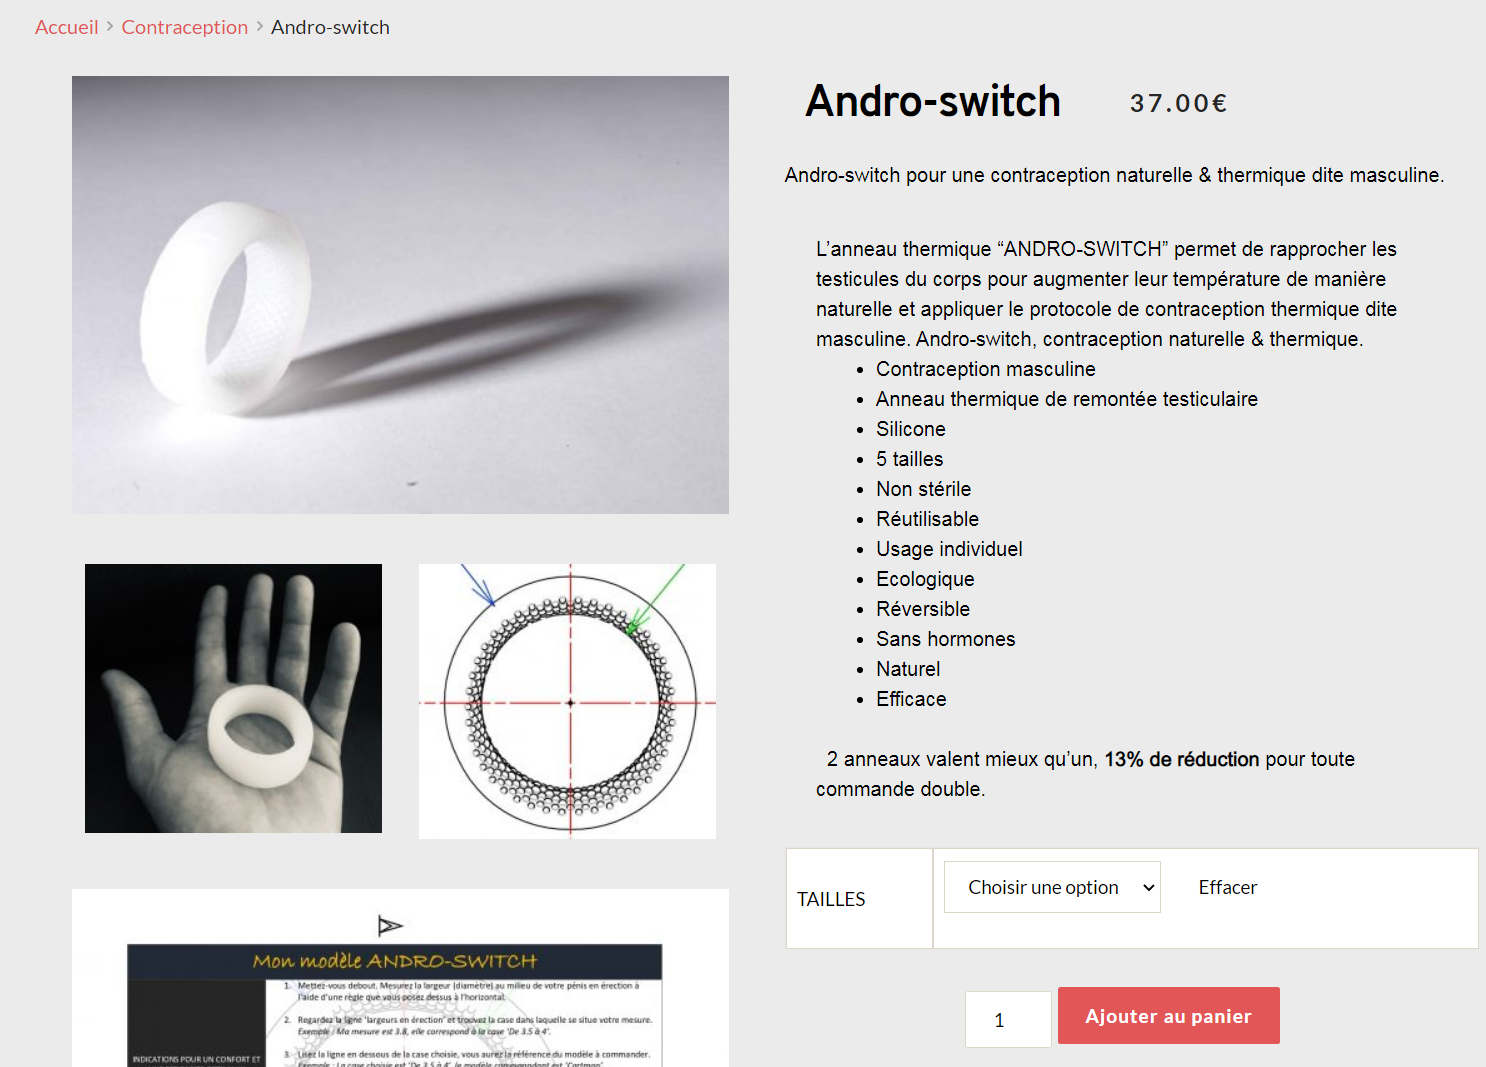
\includegraphics[width=0.5\textwidth]{images/scientiphique/vente_andro_switch.png}
    \caption{Page de vente de l'andro-switch au 13 juin 2021}
    \label{fig:vente_andro_switch}
\end{figure}

Cependant, en décembre 2021 a ordonné à Maxime Labrit de cesser la commercialisation de cet anneau, car il n'a pas passé les tests nécessaires au marquage CE. \cite{ActualiteAnneauContraceptif}

\subsection{Le gel bloquant}

Ici le principe est d'agir au niveau des canaux déférents comme le fait la vasectomie. On injecte au niveau des canaux déférents un gel qui va soit bloquer les spermatozoïdes, soit les rendre inactifs.
L'avantage de ces méthodes contrairement à la vasectomie est la possibilité d'enlever le gel pour être à nouveau fertile.
On peut par exemple citer le RISUG (Reversible Inhibition of Sperm Under Guidance) qui a passé des tests de phase 3 en Inde en 2020. \cite{ContraceptionMasculineScience}
Ainsi, lors d'une étude avec 139 participant, le RISUG a montré une efficacité de 95\% après 3 mois et 100\% après 6 mois chez les individu ayant reçu une dose de RISUG. De plus, aucun effets secondaires grave n'a été repéré et des effets secondaires benins (douleurs, gonflements) ont disparu après 1 à 6 mois après l'injection. \cite{sharmaSafetyEfficacyIntravasal2019}
On peut noter que lors d'une autre étude, il y a eu une grossesse non planifiée lié à une injection ratée. \cite{RisugWikipedia}
L'efficacité a été testé pour une durée d'au moins 10 ans, cependant, sa réversibilité n'a pour le moment pas été testé sur les humains. Elle a cependant été testé avec succès sur les animaux. \cite{khilwaniRISUGMaleContraceptive2020}

Au États-Unis, les droits du RISUG ont été acheté par Parsemus Fundation qui développait un produit dérivé : le Vasalgel. Mais récemment NEXT Life Sciences a racheté les droits du Vasalgel pour développer le: plan a. \cites{ReversibleInhibitionSperm}{VasalgelMaleContraceptive}{PlanReversibleMale}

Il s'agit actuellement d'un des contraceptifs masculin les plus avancés. \cite{ContraceptionMasculineScience}

\chapter{La contraception masculine dans la société}

\section{L'historique militant de la contraception masculine en France} \label{section:militant}

L'histoire de la contraception masculine est intimement lié au féminisme.
Nous sommes dans les années 70, la pilule contraceptive féminine est autorisé depuis 1967, la vasectomie et la ligature des trompes (stérilisation féminine) est encore interdite. \cite{guillaumedaudinContraceptesEnqueteDernier2022}{CesHommesQui}
Des hommes se retrouvent dans des groupes de paroles pour parler de la place des hommes dans la société, de masculinité.
À Paris, dans un groupe où la contraception masculine était un sujet récurrent, ils ont cherché à se contracter.

Dans leurs recherches, ils ont rencontré le médecin Jean-Claude Soufir. \cites{guillaumedaudinContraceptesEnqueteDernier2022}{HistoriqueArdecom}
Ce médecin était confronté à des patientes intolérantes à la pilule et qui ne voulait pas utiliser le stérilet comme moyen de contraception.
Il était donc à la recherche d'une méthode de contraception masculine.
Ainsi, il commença avec 6 volontaires à tester la prise de stéroïdes pour bloquer la spermatogenèse et l'application d'un gel de testostérone pour compenser la baisse.
Ces deux produits étaient déjà disponibles en pharmacie, mais n'étaient pas utilisé pour la contraception. \cites{soufirReversibleInhibitionSperm1983}{bobikaCoeurZobs2022}
Les résultats furent très positifs avec une quantité de spermatozoïde en chute et un retour à la normale après l'arrêt du traitement.
Les effets secondaires étaient les mêmes que ceux aujourd'hui connu pour la contraception hormonale, voir section \ref{effets-secondaires-methodes-hormonales}. \cite{soufirReversibleInhibitionSperm1983}
Experience qui a été par la suite reconduite dans d'autres groupes comme à Lyon. \cite{ContraceptionSeDecline1982}

Le groupe de parole a donc créé l'ARDECOM (Association pour la Recherche et le Développement de la Contraception Masculine) pour partager leur expérience à d'autres hommes.
Des antennes locales se sont créées dans plusieurs villes de France. \cites{HistoriqueArdecom}{guillaumedaudinContraceptesEnqueteDernier2022}

Ainsi, dans l'antenne locale de Toulouse, le groupe est contre la prise d'hormones.
Ils ont donc cherché d'autres méthodes de contraception masculine et ont testé la méthode thermique.
Après plusieurs tentatives, ils en ont conclu que la méthode la plus simple était celle de rapprocher les testicules du corps. \cite{bobikaCoeurZobs2022}
Ainsi au début des années 80, il y a eu au maximum 25 hommes utilisant la méthode thermique en France. \cite{guillaumedaudinContraceptesEnqueteDernier2022}

Mais, dès 1983, devant le manque de nouveaux individus et le manque d'avancé dans les méthodes de contraception, l'ARDECOM rencontre des difficultés avec des groupes locaux qui n'ont plus d'existence régulière.
De plus, en 1985 avec la pandémie du SIDA, la contraception n'est plus une priorité.
Le médecin Roger Mieusset dit qu'il a 2 ou 3 hommes qui viennent par an pour la contraception masculine. \cite{guillaumedaudinContraceptesEnqueteDernier2022}

Mais, en dans les années 2010 survient le scandale de la pilule. Ainsi en 2012 \textit{Le Monde} titre : <<Alerte sur la pilule>>.
En effet, les pilules de 3\textsuperscript{ème} et 4\textsuperscript{ème} génération augmentent le risque de Thrombose veineuse, ce qui peut mener à un AVC.
Ainsi un rapport de l'agence du médicament en 2013 conclu qu'en France, la pilule provoque 2 529 accidents thromboemboliques veineux et 20 décès prématurés.
Suite à ce scandale, les femmes ont voulu trouver une alternative à la pilule. \cites{albrechtQuelleEstPlace2023}{guillaumedaudinContraceptesEnqueteDernier2022}{AlertePilule2012}

C'est ainsi que la contraception masculine a regagné de l'intérêt. Ainsi, le médecin Roger Mieusset qui voyait 5 hommes par an en 2012 pour une contraception masculine en voit environ 90 par an en 2020.\cite{guillaumedaudinContraceptesEnqueteDernier2022}
Il est actuellement le seul médecin en France à prescrire la contraception avec un slip chauffant.\cite{bobikaCoeurZobs2022}
De plus, en 2015, Lydie Porée est devenue référente sur la contraception masculine au planning familial.
Mais, elle n'avait aucunes connaissances sur la contraception masculine.
Mais depuis 2016, le planning familial mets l'accent dessus, des médecins en France sont formé et des réunions sont organisé à Paris chaque premier samedi du mois spécialement pour la contraception masculine.
Cependant, Lydie Porée dit qu'il leur arrive de faire des réunions quasiment vides. \cite{guillaumedaudinContraceptesEnqueteDernier2022}

De plus, on peut noter l'émergence d'autres initiatives telle que l'association \textit{GARCON} \cite{QuiSommesNous}, le collectif \textit{Thomas Bouloù} \cite{ThomasBoulouInterview} ou les BD: \textit{Les Contraceptés enquête sur le derier tabou} de Guillaume Daudin, Stéphane Jourdain et Caroline Lee \cite{guillaumedaudinContraceptesEnqueteDernier2022} et \textit{Le coeur des Zobs} de Bobika \cite{bobikaCoeurZobs2022} et les ateliers créé dans de multiples villes en France. \cites{ContraceptionMasculineComment2023}{OuNousTrouver}{guillaumedaudinContraceptesEnqueteDernier2022} visant à faire connaitre la contraception masculine et à la rendre plus accessible.

\section{L'acceptation dans la société}

Est-ce que ce milieu militant est représentatif de la société ?

\subsection{Sondage communauté UTBM}
Pour répondre à cette question, j'ai réalisé un sondage que j'ai diffusé au courant du mois de mars au sein de l'Université de Technologie de Belfort et sur mes réseaux sociaux. 369 personnes ont répondu au sondage.

Avant d'analyser les résultats, il faut note que ce sondage a été effectué au sein d'un milieu universitaire avec majoritairement des jeunes de 18 à 25 ans:

\begin{table*}[H]
    \centering
    \begin{tabular}{|l|c|}
    \hline
    \textbf{Groupe d'âge} & \textbf{Nombre de réponses} \\
    \hline
    Moins de 18 ans & 3 \\
    18 à 25 ans & 310 \\
    25 à 35 ans & 17 \\
    35 à 50 ans & 29 \\
    50 à 70 ans & 10 \\
    Plus de 70 ans & 0 \\
    \hline
    \end{tabular}
    \caption{Groupe d'âge}
\end{table*}
    
\begin{table}[H]
    \centering
    \begin{tabular}{|l|c|}
    \hline
    \textbf{Profession} & \textbf{Nombre de réponses} \\
    \hline
    Étudiant & 300 \\
    Agriculteur & 0 \\
    Artisan, commerçant ou chef d'entreprise & 1 \\
    Cadre & 25 \\
    Employé & 40 \\
    Ouvrier & 2 \\
    Retraité & 1 \\
    \hline
    \end{tabular}
    \caption{Profession}
    \label{tab:Profession}
\end{table}

De plus, il faut noter que pour toutes les prochaines réponses, les personnes pouvaient ne pas répondre.
Ce choix a été fait pour éviter qu'une personne arrête le test, car une question était trop privée.

De plus, on note que la répartition entre les personnes de sexe féminin et masculin est la suivante :

\begin{table}[H]
    \centering
    \begin{tabular}{|l|c|c|}
    \hline
    \textbf{Genre} & \textbf{Nombre} & \textbf{Pourcentage (\%)} \\
    \hline
    Masculin & 206 & 55.83 \\
    Féminin & 163 & 44.17 \\
    \hline
\end{tabular}
\caption{Répartition des personnes de sexe féminin et masculin}
\end{table}

Ainsi, on peut voir que la répartition est assez équilibrée. Cependant, il faut noter que le nombre de personnes de sexe féminin est très inférieur dans les étudiant de l'UTNM.
En effet, il y a 18\% de personnes de sexe féminin à l'UTBM. \cite{UTBMClassementEcoles}
Et, bien que dans le personnel la répartition est équilibrée \cite{RapportSocial20202020}, la majorité des réponses venants d'étudiant (voir tableau \ref{tab:Profession}), la répartition est proprtiellement déséquilibrée.
On peut donc imaginer que les personnes de sexe féminin sont plus intéressé par la contraception que celles de sexe masculin.

Une des questions de ce test était: "Quels moyens de contraception masculine connaissez-vous ?"

À cette réponse, on peut voir plusieurs choses intéressantes :
\begin{itemize}
    \item Bien que le préservatif soit le plus cité, on peut voir qu'il ne l'est pas systématiquement. En effet, en discutant avec Loïc Rueff, infirmier à l'UTBM, il m'a dit que le préservatif n'était plus majoritairement vu comme un moyen de protection, mais comme un moyen de protection des MST suite aux campagnes de prévention.
    \item La vasectomie est citée par 31\% des répondants.
    \item La méthode thermique est cité par quelques participants.
    \item Plusieurs personnes ont cité la pilule en précisant qu'elle était encore au stade expérimental.
\end{itemize}

Par la suite, il a été demandé aux personnes de sexe masculin si elles utilisaient un moyen de contraception masculine, 118 des 203 réponses ont répondu par l'affirmative.

Paris ces 118 personnes 117 personnes ont donné leur moyen de contraception. L'écrasante majorité utilise le préservatif.
3 ont cité l'anneau et 2 le retrait.

Ensuite, il a été demandé aux personnes de sexe masculin de juger leur niveau de connaissances, de confiance et de possibilité d'utilisation pour une sélection de méthode de contraception masculine.

Les résultats sont les suivants:



\begin{table}[ht]
\centering
\renewcommand\theadfont{\normalsize\bfseries}
\renewcommand\theadalign{cc}
\begin{tabular}{|l|c|c|c|c|}
\hline
\thead{Méthode} & \thead{Connaissances} & \thead{Confiance} & \thead{Probabilité\\ d'utilisation} & \thead{Efficacité\\ pratique (\%)} \\
\hline
Préservatif & 6,9 & 8,43 & 6,87 & 85\% \\
Vasectomie & 3,92 & 8,54 & 3,16 & 99,80\% \\
Retrait & 6,19 & 2,05 & 2,03 & 78\% \\
Méthode hormonale & 2,78 & 5,56 & 3,68 & - \\
Méthode thermique & 3,57 & 4,17 & 3,15 & - \\
\hline
\end{tabular}
\caption{Réponses des personnes de sexe masculin sur leur niveau de connaissances, de confiance et de possibilité d'utilisation pour une sélection de méthode de contraception masculine}
\end{table}

    

Ainsi, on peut voir que les personnes de sexe masculin considère qu'elles ont bonne connaissance du préservatif et de la vasectomie, mais beaucoup moins des autres.
Cependant avoir une connnaissance moyenne de la vasectomie n'empêche pas d'avoir une confiance élevée en celle-ci.
Cependant, on peut voir que les gens ont une très grande confiance envers le préservatif (8.43) mais une très petite avec le retrait (2.05) alors que leur scores d'efficacités réelle n'ont que 6 points d'écarts
De plus, on peut noter que les gens ont peu confiance en la méthode hormonale alors que lors des études, elle a démontré une plus grande efficacité que le préservatif. \cite{abbeMaleContraception2020}

De plus, on peut voir que la seule méthode avec une forte probabilité d'utilisation est uniquement le préservatif, malgré une grande confiance envers la vasectomie. Le caractère définitif de la vasectomie rebutant probablement les potentiels utilisateurs.

La question de la confiance a aussi été demandé aux personnes de sexe féminin, avec les réponses suivantes:


\begin{table}[ht]
\centering
\renewcommand\theadfont{\normalsize\bfseries}
\renewcommand\theadalign{cc}
\begin{tabular}{|l|c|} \label{table:confiance_par_moyen}
\hline
\thead{Méthode} & \thead{Confiance} \\
\hline
Préservatif & 8,05 \\
Vasectomie & 8,23 \\
Retrait & 1,74 \\
Méthode hormonale & 5,95 \\
Méthode thermique & 4,05 \\
\hline
\end{tabular}
\caption{Niveau de confiance pour différentes méthodes de contraception masculin pour les personnes de sexe féminin}
\end{table}

Ainsi, les scores sont très proches, on peut noter que les personnes de sexe féminin font très légèrement moins confiance aux méthodes de contraceptions masculine que les hommes, à l'exception de la méthode hormonale où elles font un peu plus confiance. Cependant, l'échantillon et l'écart sont faibles, ces résultats ne peuvent donc pas être considérés comme une vérité générale.

De plus, lors du questionnaire, j'ai demandé aux hommes de décrire en quelques mots chacune des méthodes de contraception, voici les tendances qui en ressortent :

\begin{itemize}
    \item \textbf{Préservatif} : Beaucoup de personnes parlent des MST avec raison dans leurs réponses. De plus, il y a plusieurs réponses qui disent que le préservatif est contraignant ou désagréable. Il y a aussi eu quelques réponses appuyant qu'il s'agissait du moyen de contraception parfait pour les relations éphémères. Ce que m'a confirmé Loïs Rueff, en effet, il s'agit de la seule à protéger des MST quand les partenaires ne se sont pas testé.
    
    \item \textbf{Vasectomie} : Les réponses ont beaucoup appuyé le côté définitif de la vasectomie. Il faut rappeler qu'elle est potentiellement inversible, mais ça reste une opération complexe. Dans ces réponses, on peut aussi lire beaucoup d'allusion à de la mutilation ou des réponses très épidermique telle que : "Une honte pour tout homme qui se respecte."
    On voit par là que la vasectomie est un moyen de contraception complexe, avec des personnes ayant de fortes opinions.
    
    \item \textbf{Le retrait} : Les réponses décrivent sans problème le retrait. Beaucoup de réponses insistent sur le fait que ce n'est pas fiable ou que ce n'est pas une méthode de contraception. Le retrait est techniquement une méthode de contraception, cependant elle n'est pas fiable avec un risque élevé de grosses (voir section \ref{section:leretrait}). L'infirmier de l'UTBM ainsi que toutes les ressources gouvernementales le déconseille formellement.

    \item \textbf{La contraception hormonale} : Avant d'analyser les réponses, il est intéressant de noter qu'il n'y a eu que 115 réponses pour cette méthode contrairement au préservatif avec 140 réponses. Dans les réponses, on peut noter que beaucoup de personnes ne connaissent pas, ce qui est confirmé par leur propre évaluation de connaissance sur le sujet avec une moyenne de 2.78 sur 10. Beaucoup de personnes évoque la pilule et la compare à la pilule pour femme. De plus, on peut voir que la méfiance grimpante envers la pilule pour femme \cite{albrechtQuelleEstPlace2023} touche aussi la contraception hormonale. Chose qui m'a été confirmé par des personnes de sexe féminin à qui j'ai parlé qui m'ont entre autres dit : "La pilule pour homme, je ne vous la souhaite pas". On peut aussi voir que beaucoup de personnes parlent des articles que l'on peut régulièrement lire parlant d'expérimentations et d'une pilule disponible dans les futures années. Enfin, peu de personnes évoquent la contraception hormonale avec les injections qui est pour autant la seule contraception hormonale que l'OMS a considérée comme fiable. (voir section \ref{section:injection})

    \item \textbf{La contraception thermique} : On peut aussi noter un plus faible niveau de réponses avec 116 réponses. Dans les réponses, on remarque aussi beaucoup de personnes qui ne connaissent pas cette méthode et qui se posent des questions. On peut cependant voir que certaines personnes la connaissent très bien et font de longues descriptions pour bien l'expliquer. De plus, plusieurs personnes évoquent la gène potentiel, l'organisation à avoir et la peur d'effectuer des erreurs. De plus, on peut noter plusieurs personnes considère cette méthode saine ou bien naturelle. Cependant, plusieurs personnes relève aussi qu'elle n'a pas été testé, qu'elle n'est pas fiable, ou n'y croient pas. Bien que cette méthode ne soit ni validé par l'OMS ni par le ministère de la Santé, l'Association française d'urologie l'a validé. (Voir section : \ref{section:thermique})
    
\end{itemize}

Par la suite, il a été demandé aux personnes de sexe masculin: <<Sur une échelle de 1 (peu probable) à 5 (probable) seriez vous prêts accepter les effets secondaires d'une méthode de contraception s'il y a : >>

\begin{figure}[H]
    \centering
    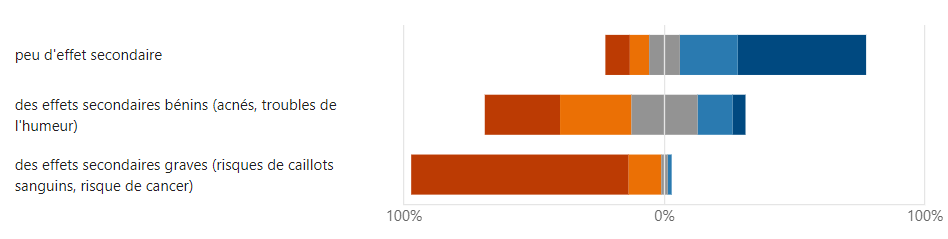
\includegraphics[width=1\textwidth]{images/questionnaire/Acceptation effets secondaires.png}
    \caption{Réponses en fonction des effets secondaires}
    \label{fig:reponse_effets_secondaires}
\end{figure}

Il est intéressant de noter que les exemples mis à côté des effets secondaires sont tous des effets secondaires de la pilule féminine.

Maintenant en comparant ça avec les réponses à la question suivante : <<Seriez-vous prêts à prendre une contraception hormonale s'il y a les mêmes effets secondaires que ceux d'une pilule pour femme ?>>

\begin{table}[H]
\centering
\begin{tabular}{|l|c|c|}
\hline
\textbf{Réponse} & \textbf{Nombre} & \textbf{Pourcentage (\%)} \\
\hline
Oui & 99 & 50.77\% \\
Non & 96 & 49.23\% \\
\hline
\end{tabular}
\caption{Acceptation des effets secondaires de la pilule féminine pour les personnes de sexe masculin}
\end{table}

On peut ainsi voir que quand on dit aux personnes de sexe masculin qu'il y a un risque de caillot sanguin ou de cancer, ils sont peu enclins à prendre une méthode de contraception. Alors que quand on dit qu'il s'agit des mêmes effets secondaires que la pilule féminine, ils sont bien plus enclins à la prendre. Les caillots sanguins et le cancer étant un effet secondaire potentiel de la pilule, ces réponses sont dissonantes. Les hypothèses que j'ai pour expliquer ces réponses :
\begin{itemize}
    \item Une méconnaissance des effets de la pilule.
    \item Une partie que se dit que si les personnes de sexe féminin le font, ils peuvent aussi le faire.
\end{itemize}
Un questionnaire avec des questions plus spécifique serait nécessaire pour évaluer ces hypothèses.

Il a été demandé aux personnes de sexe féminin sur une échelle de 1 à 10 si elles pensaient que les hommes devaient s'intéresser à la contraception. Avec une moyenne à 9.84 et un minimum à 7 sur les 163 réponses, on peut voir que les personnes de sexe féminin ont envie que les hommes s'y intéressent.

Par la suite, la confiance envers un homme contracepté a été questionner. Les réponses pour chaque moyen de comparaison ont déjà été étudiés dans le tableau \ref{table:confiance_par_moyen}. De plus, il a été aussi demandé leur confiance en fonction de la situation relationnelle qu'ils ont avec leur partenaire :

\begin{table}[ht]
\centering
\begin{tabular}{|l|c|}
\hline
\textbf{Situation relationnelle} & \textbf{Confiance} \\
\hline
Relation d'un soir & 3,11 \\
En couple & 8,38 \\
\hline
\end{tabular}
\caption{Confiance en fonction de la situation relationnelle}
\end{table}

De plus, il est important de noter que pour une relation d'un soir, le préservatif est le seul moyen de se protéger des MST. Mais, on voit que dans le cas d'un couple, la relation est importante, ce qui est nécessaire, en particulier quand en cas d'erreur, c'est la personne de sexe féminin qui sera enceinte et qui devra, si elle ne veut pas d'enfant, prendre une pilule du lendemain ou avorter.

Par la suite, tous les participants ont dû évaluer sur une échelle de 1 à 10 les informations qu'ils ont eues sur la contraception par différents acteurs :

\begin{table}[ht]
\centering
\begin{tabular}{|l|c|c|}
\hline
Niveau d'information & \textbf{Contraception} & \textbf{Contraception masculine} \\
\hline
Cours d'éducation sexuelle & 4,31 & 2,49 \\
Médecin & 3,42 & 1,9 \\
\hline
\end{tabular}
\caption{Niveau d'information sur la contraception}
\end{table}

On peut noter que quelle que soit la source d'information ou le type de contraception, les valeurs sont toujours en dessous de 5, ce qui est faible. De plus, les personnes ont plus l'impression de ne pas avoir été assez informer sur la contraception masculine que la contraception en général.

Enfin, il a été demandé aux participants d'évaluer selon le sexe la nécessiter de participation dans la contraception :

\begin{table}[ht]
\centering
\begin{tabular}{|l|c|}
\hline
\textbf{Groupe} & \textbf{Niveau} \\
\hline
Les femmes & 3,59 \\
Les hommes & 3,99 \\
Discussions des partenaires & 9,75 \\
\hline
\end{tabular}
\caption{Évaluation selon le sexe de la nécessiter de participation dans la contraception}
\end{table}

On peut voir que les participants considère très majoritairement que la contraception doit être un sujet de discussion et non géré par un seul des membres du couple.

\section{La contraception masculine dans les médias}

\subsection{La contraception masculine vu à la télévision}

Dès 1973, un professeur apparait à la télévision dans une émission produite par l'ORTF pour parler de contraception masculine. Il parle beaucoup de la vasectomie, mais ne la considère pas comme une méthode contraceptive satisfaisante, car la vasectomie n'est pas réversible dans 100 \%. De plus, il pense que la vasectomie ne sera pas effectuée à grande échelle, car en France il y a des préjugées : "Tout ce qui touche aux organes génitaux de l'homme, c'est sacré, la femme, on peut y toucher, mais l'homme oulalal". Deux téléspectateurs avaient été amené sur le plateau et étaient tous deux favorable à la vasectomie. \cite{ProfesseurNetterContraception} Rappelons qu'à cette époque la vasectomie n'était pas légal. \cite{guillaumedaudinContraceptesEnqueteDernier2022} De plus, plus tard dans l'émission, en parlant de la pilule, il évoque le fait que les hommes, si on leur dit qu'ils n'auront plus de spermatozoïdes, ils penseront que ça va les rendre impuissant et ainsi, la pilule pour homme ne sera pas démocratisé prochainement. \cite{inaactuPilulePourHomme2019}

En effet, on peut voir dans un micro trottoir diffusé dans les années 1981, où un homme en parlant de contraception considère que ça toucherait son identité d'homme : <<Jamais. Je ne veux pas. Parce que l'homme doit rester homme toute la vie>>. De plus, lors de la même émission, on peut voir que les femmes demandent s'il n'existe pas des moyens de contraception pour les hommes. Cependant, la majorité des personnes interrogée lors de micro trottoir se disent favorables à la pilule pour homme. \cites{MicrotrottoirHommesPour}{PilulePourHomme}

Dans les années 80, il y a eu plusieurs passages à la télé avec des membres de l'ARDECOM où ils présentaient leur expérience avec la pilule pour homme. (voir section \ref{section:militant}) Dans ces émissions, il leur a souvent été posé la question des effets secondaires, la comparaison avec la pilule féminine. De plus, ils évoquèrent souvent qu'il s'agissait d'un choix militant et qu'ils voulaient : <<Partager la responsabilité de la contraception avec leur partenaire>> \cites{inaactuPilulePourHomme2019}{1980HommeVient}

Campagne de préventions

Préservatif

Dans combien de temps ça sera disponible

En parallèle, on peut voir que lors des campagnes de préventions pour la cont



\listoffigures

\begin{appendix}

    \chapter{Les étapes de la recherche} \label{annexe:etapes_recherche}

    Pour mieux comprendre l'état actuel de la recherche, il faut d'abord comprendre comment est développé un médicament.
Le développement d'un médicament est divisé en plusieurs phases: \cite{DeveloppementMedicamentInserm}

\begin{itemize}
    \item Recherche fondamentale : Il s'agit de la première étape de la recherche.
    Lors de cette étape on cherche des molécules candidates pour être utilisées comme médicament.
    On va analyser la réaction de ces molécules sur des cellules ou des tissus.
    On va sélectionner les meilleurs candidats, essayer d'améliorer leurs propriétés.

    \item Recherche préclinique : Lors de cette étape on va tester les molécules candidates sur des animaux.
    On va regarder comment elles réagissent sur des animaux, analyser s'il n'y a pas des effets secondaires, effectuer une première estimation des dosages pour l'humain.

    \item Évaluation clinique : Lors de cette étape on va tester les molécules candidates sur des humains.

    \begin{itemize}
        \item Phase 1 : On va tester la sécurité des molécules candidates sur des humains. Ici on ne teste pas l'efficacité, mais on va regarder comment elles agissent sur le corps ou si elles sont dangereuses. Les tests sont effectués sur des volontaires sains.
        \item Phase 2 : On va tester les molécules candidates sur des patients atteints de la maladie pour laquelle on cherche un médicament. De plus, plusieurs dosages seront testés pour voir lequel est le plus efficace tout en limitant les effets secondaires.
        \item Phase 3 : On va tester les molécules sur des patients malades afin d'évaluer l'efficacité du médicament. Pour cela il faut comparer l'efficacité entre les patients qui ont pris le médicament et ceux qui ont pris un placebo. Ceci permet de voir si le médicament est réellement efficace ou s'il s'agit que de l'effet placebo. En effet l'effet placebo est très puissant et peut faire croire à l'efficacité d'un médicament alors qu'il n'en a pas. \cite{decraenPlacebosPlaceboEffects1999} Cette étape dure souvent plusieurs années.
    \end{itemize}

    \item L’autorisation de mise sur le marché (AMM) : Lors de cette étape, le laboratoire qui veut commercialiser une molécule doit demander l'autorisation de la mettre sur le marché. Pour cela il faut démontrer que le médicament est efficace et sûr. L'AMM est délivrée par l'Agence nationale de sécurité du médicament et des produits de santé (ANSM). Cette étape dure au minimum 1 an.
    \item Une fois l'AMM obtenue, le laboratoire peut commercialiser le médicament. Cependant, le médicament continue d'être surveillé au travers des retours du personnel médical, par exemple pour détecter des effets secondaires très rares.
\end{itemize}

Au total, entre le moment où une molécule est identifié par la recherche fondamentale et mis sur le marché il peut s'écouler au moins 10 ans. \cite{DeveloppementMedicamentInserm} Du plus, a chaque étape la molécule peut être abandonnée et la recherche repart du début. \cite{denisvanwaerebekeJamesOuRoman2018}

\end{appendix}

\printbibliography

\end{document}

